%%%%%%%%%%%%%%%%%%%%%%%%%%%%%%%%%%%%%%%%%%%%%%%%%%%%%%%%%%%%%%%%%%%%%%%%%%%%%%%%
% TUM-Vorlage: Wissenschaftliche Arbeit
%%%%%%%%%%%%%%%%%%%%%%%%%%%%%%%%%%%%%%%%%%%%%%%%%%%%%%%%%%%%%%%%%%%%%%%%%%%%%%%%
%
% Rechteinhaber:
%     Technische Universität München
%     https://www.tum.de
% 
% Gestaltung:
%     ediundsepp Gestaltungsgesellschaft, München
%     http://www.ediundsepp.de
% 
% Technische Umsetzung:
%     eWorks GmbH, Frankfurt am Main
%     http://www.eworks.de
%
%%%%%%%%%%%%%%%%%%%%%%%%%%%%%%%%%%%%%%%%%%%%%%%%%%%%%%%%%%%%%%%%%%%%%%%%%%%%%%%%


%%%%%%%%%%%%%%%%%%%%%%%%%%%%%%%%%%%%%%%%%%%%%%%%%%%%%%%%%%%%%%%%%%%%%%%%%%%%%%%%
\documentclass[%
    fontsize=11pt, % Schriftgröße
    twoside=off % kein einseitiges Layout
]{scrbook} % Dokumentenklasse: KOMA-Script Book
\usepackage{scrlayer-scrpage} % Anpassbare Kopf- und Fußzeilen

\usepackage[utf8]{inputenc} % Textkodierung: UTF-8
\usepackage[T1]{fontenc} % Zeichensatzkodierung

\usepackage[ngerman]{babel} % Deutsche Lokalisierung
\usepackage{graphicx} % Grafiken

% Schriftart Helvetica:
\usepackage[scaled]{helvet}
\renewcommand{\familydefault}{\sfdefault}

% Silbentrennung:
\usepackage{hyphenat}
\hyphenation{TUM in-te-res-siert} % Eigene Silbentrennung
%\tolerance 2414
%\hbadness 2414
%\emergencystretch 1.5em
%\hfuzz 0.3pt
%\widowpenalty=10000     % Hurenkinder
%\clubpenalty=10000      % Schusterjungen
%\vfuzz \hfuzz

\usepackage[hidelinks]{hyperref} % Hyperlinks
\usepackage[onehalfspacing]{setspace} % 1,5facher Zeilenabstand
\usepackage{calc} % Berechnungen
\usepackage{enumitem} % Mehr Kontrolle über itemize-, enumerate- und description-Umgebungen
\usepackage{relsize} % Schriftgröße in Abhängigkeit von aktueller anpassen
\usepackage{tabularx} % Flexiblere Tabellen
\usepackage{caption} % Anpassen von Beschriftungen

% Nummerierung von Abbildungen & Tabellen durchgängig, statt nach Kapiteln:
\usepackage{chngcntr}
\counterwithout{figure}{chapter}
\counterwithout{table}{chapter}

% Abkürzungen, Glossare:
\usepackage[%
    xindy,% xindy zum Indexieren verwenden
    acronym,% Separates Akronym-Verzeichnis
    nopostdot,% Kein Punkt am Ende einer Beschreibung im Glossar
]{glossaries}

% Spezielle Befehlsdefinitionen:
\newcommand{\Thema}{}

% Debugging:
%\usepackage{showframe} % Layout-Boxen anzeigen
%\usepackage{layout} % Layout-Informationen
%\usepackage{printlen} % Längenwerte ausgeben
 % !!! NICHT ENTFERNEN !!!
%%%%%%%%%%%%%%%%%%%%%%%%%%%%%%%%%%%%%%%%%%%%%%%%%%%%%%%%%%%%%%%%%%%%%%%%%%%%%%%%

\renewcommand{\Thema}{%    Competition as a driving motivational factor for gamification purposes
                        Wettbewerb als treibende Motivation in Gamification Kontexten}


%%%%%%%%%%%%%%%%%%%%%%%%%%%%%%%%%%%%%%%%%%%%%%%%%%%%%%%%%%%%%%%%%%%%%%%%%%%%%%%%
%%%%%%%%%%%%%%%%%%%%%%%%%%%%%%%%%%%%%%%%%%%%%%%%%%%%%%%%%%%%%%%%%%%%%%%%%%%%%%%%
% EINSTELLUNGEN
%%%%%%%%%%%%%%%%%%%%%%%%%%%%%%%%%%%%%%%%%%%%%%%%%%%%%%%%%%%%%%%%%%%%%%%%%%%%%%%%

\KOMAoptions{parskip=full}


% Seitenränder:

\newcommand{\SeitenrandOben}{25.8mm}
\newcommand{\SeitenrandRechts}{21mm}
\newcommand{\SeitenrandLinks}{40mm}
\newcommand{\SeitenrandUnten}{24.8mm}
\newcommand{\FusszeileHoehe}{11.7mm}

\usepackage[a4paper,
    head=0pt,
    top=\SeitenrandOben,
    bottom=\SeitenrandUnten,
    inner=\SeitenrandLinks,
    outer=\SeitenrandRechts
]{geometry}


% Fußzeilen:

\setlength{\footheight}{\FusszeileHoehe}
\clearscrheadfoot
\ifoot*{\Thema\vfill}
\ofoot*{\pagemark\vfill}
\setkomafont{pageheadfoot}{\fontsize{9pt}{13pt}\normalfont}
\setkomafont{pagefoot}{\bfseries}
\setkomafont{pagenumber}{\normalfont}
\pagestyle{scrheadings}


% Fußnoten:

\KOMAoptions{%
    footnotes=multiple % mehrere Fußnoten werden durch Zeichen getrennt
}
%\setfootnoterule[.6pt]{5.08cm}
\renewcommand{\footnoterule}{\hrule width 5.08cm height .6pt \vspace*{3.9mm}}
%\setlength{\footnotesep}{5mm}
\deffootnote{2mm}{2mm}{%
    \makebox[2mm][l]{\textsuperscript{\thefootnotemark}}%
}
\setkomafont{footnoterule}{\fontsize{9pt}{20pt}\selectfont}


% Überschriften:

\KOMAoptions{%
    open=any, % keine Festlegung auf linke oder rechte Seite
    numbers=noendperiod, % kein automatischer Punkt nach Gliederungsnummer
    headings=small
}

\makeatletter
\g@addto@macro{\@afterheading}{\vspace{-\parskip}} % \parskip nach Gliederungsbefehlen entfernen
\renewcommand*{\chapterheadstartvskip}{\vspace{\@tempskipa}\vspace{-3pt}} % Korrektur für Abstand über Kapitelüberschriften
\makeatother

\setkomafont{disposition}{\normalfont\sffamily}

\setkomafont{chapter}{\normalfont\fontsize{19pt}{22pt}\selectfont}
\RedeclareSectionCommand[%
  beforeskip=0pt,
  afterskip=29pt
]{chapter}
\renewcommand*{\chapterformat}{\thechapter.\enskip} % Immer Punkt nach Kapitelnummer

\setkomafont{section}{\fontsize{15pt}{17pt}\selectfont}
\RedeclareSectionCommand[%
  beforeskip=0pt,
  afterskip=24.1pt
]{section}
\renewcommand*{\sectionformat}{\makebox[13mm][l]{\thesection.\enskip}} % Feste Breite für Abschnittsnummer und immer Punkt danach

\setkomafont{subsection}{\bfseries\fontsize{12pt}{13pt}\selectfont}
\RedeclareSectionCommand[%
  beforeskip=0pt,
  afterskip=1pt
]{subsection}
\renewcommand*{\subsectionformat}{\makebox[13mm][l]{\thesubsection.\enskip}} % Feste Breite für Unterabschnittsnummer und immer Punkt danach


% Listen:

\setlist{%
    labelsep=0mm,
    itemindent=0pt,
    labelindent=0pt,
    align=left,
    parsep=1.5ex
}
\setlist[itemize]{%
    leftmargin=5mm,
    labelwidth=4.9mm
}
\setlist[itemize,1]{%
    before={\vspace{0.25ex}},
    label={\raisebox{.35ex}{\smaller[2]\textbullet}},
    after={\vspace{-\parsep}\vspace{-.25ex}}
}
\setlist[itemize,2]{%
    label={\raisebox{.35ex}{\rule{.58ex}{.58ex}}}
}
\setlist[enumerate]{%
    leftmargin=10mm,
    labelwidth=9.9mm
}
\setlist[enumerate,2]{%
    label={\alph*.}
}

\setlist[description]{%
%    labelindent=!,
    leftmargin=1em,
    labelwidth=!,
    parsep=0mm,
    partopsep=0mm,
    labelsep=1em,
}


% Verzeichnisse:

\KOMAoptions{%
    %toc=flat, % keine Einrückungen im Inhaltsverzeichnis
    toc=chapterentrydotfill, % Punkte bis zur Seitennummer bei Kapiteln
    listof=entryprefix, % Präfix für Einträge in Abbildungs- und Tabellenverzeichnis
    listof=nochaptergap, % Kein Abstand für Kapiteleinträge in extra Verzeichnissen
}

\makeatletter
\renewcommand{\@dotsep}{.3} % Abstand der Füllpunkte

% "chapteratlist" für Inhaltsverzeichnis auswerten:
\renewcommand*{\addchaptertocentry}[2]{%
  \iftocfeature{toc}{chapteratlist}{}{%
    \addtocontents{toc}{\protect\vspace{-10pt}}% extra Abstand vor Kapitelüberschriften in Inhaltsverzeichnis entfernen
  }%
  % Originaldefinition aus scrbook.cls:
  \addtocentrydefault{chapter}{#1}{#2}%
  \if@chaptertolists
    \doforeachtocfile{%
      \iftocfeature{\@currext}{chapteratlist}{%
        \addxcontentsline{\@currext}{chapteratlist}[{#1}]{#2}%
      }{}%
    }%
    \@ifundefined{float@addtolists}{}{\scr@float@addtolists@warning}%
  \fi%
}
\makeatother

\AfterTOCHead[toc]{\protect\vspace{.8ex}} % Abstand zwischen Überschrift und Inhaltsverzeichnis
\setuptoc{toc}{noparskipfake} % Angleichung der Abstände nach Inhaltsverzeichnisüberschrift an andere Überschriften
\unsettoc{toc}{chapteratlist} % kein Abstand vor Kapiteleinträgen im Inhaltsverzeichnis, funktioniert nur durch obige Redefinition von \addchaptertocentry

% -- Abbildungs- und Tabellenverzeichnis:

\AfterTOCHead[lof]{\protect\vspace{-.1ex}\doublespacing} % Abstand zwischen Überschrift und Abbildungsverzeichnis, doppelter Zeilenabstand
\setuptoc{lof}{noparskipfake} % Angleichung der Abstände nach Abbildungsverzeichnisüberschrift an andere Überschriften

\AfterTOCHead[lot]{\protect\vspace{-.1ex}\doublespacing} % Abstand zwischen Überschrift und Tabellenverzeichnis, doppelter Zeilenabstand
\setuptoc{lot}{noparskipfake} % Angleichung der Abstände nach Tabellenverzeichnisüberschrift an andere Überschriften

% Beschriftungen:
\DeclareCaptionFormat{WissenschaftlicheArbeiten}{\fontsize{8pt}{10pt}\selectfont#1 #2#3\par}
\DeclareCaptionLabelFormat{WissenschaftlicheArbeiten}{\bfseries\selectfont#1 #2}

% -- Tabellen:
\captionsetup[table]{%
    format=WissenschaftlicheArbeiten,
    labelformat=WissenschaftlicheArbeiten,
    labelsep=none,
    singlelinecheck=off,
    justification=raggedright,
    skip=3pt,
    tablewithin=none
}

% -- Abbildungen:
\captionsetup[figure]{%
    format=WissenschaftlicheArbeiten,
    labelformat=WissenschaftlicheArbeiten,
    labelsep=none,
    singlelinecheck=off,
    justification=raggedright,
    skip=6.6mm,
    figurewithin=none
}


% Tabellen:
\renewcommand{\arraystretch}{1.8} % Skalierung der Tabellen
\newcolumntype{M}{X<{\vspace{4pt}}} % Spaltentyp mit Abstand rechts


% Glossare & Abkürzungsverzeichnis:

\makeglossaries
\newacronym{abk}{Abk.}{Abkürzungen}
\newacronym{bez}{Bez.}{Bezeichnung}
\setacronymstyle{short-long}

\makeatletter
\newlength{\@glsdotsep}
\setlength{\@glsdotsep}{\@dotsep em}
\newcommand*{\glsdotfill}{\leavevmode \cleaders \hb@xt@ \@glsdotsep{\hss .\hss }\hfill \kern \z@}
\makeatother

\newglossarystyle{WissenschaftlicheArbeiten}{%
  \setglossarystyle{index}%

  \renewcommand*{\glossaryheader}{\vspace{.75em}}%
  \renewcommand*{\glstreenamefmt}[1]{##1}%
  \renewcommand*{\glossentry}[2]{%
     \item\glsentryitem{##1}\glstreenamefmt{\glstarget{##1}{\glossentryname{##1}}}%
     \ifglshassymbol{##1}{\space(\glossentrysymbol{##1})}{}%
     \space-\space\glossentrydesc{##1}\glsdotfill\glspostdescription\space ##2%
  }%
  \renewcommand*{\glsgroupheading}[1]{%
    \item\glstreenamefmt{\textbf{\fontsize{14}{17}\selectfont\enskip\glsgetgrouptitle{##1}}}\vspace{.3em}}%
}

\setglossarystyle{WissenschaftlicheArbeiten}


 % !!! NICHT ENTFERNEN !!!
%%%%%%%%%%%%%%%%%%%%%%%%%%%%%%%%%%%%%%%%%%%%%%%%%%%%%%%%%%%%%%%%%%%%%%%%%%%%%%%%

\begin{document}
\bibliographystyle{unsrt}
\title{\Thema}
\author{Jeff-Owens Iyalekhue}
\date{Datum}

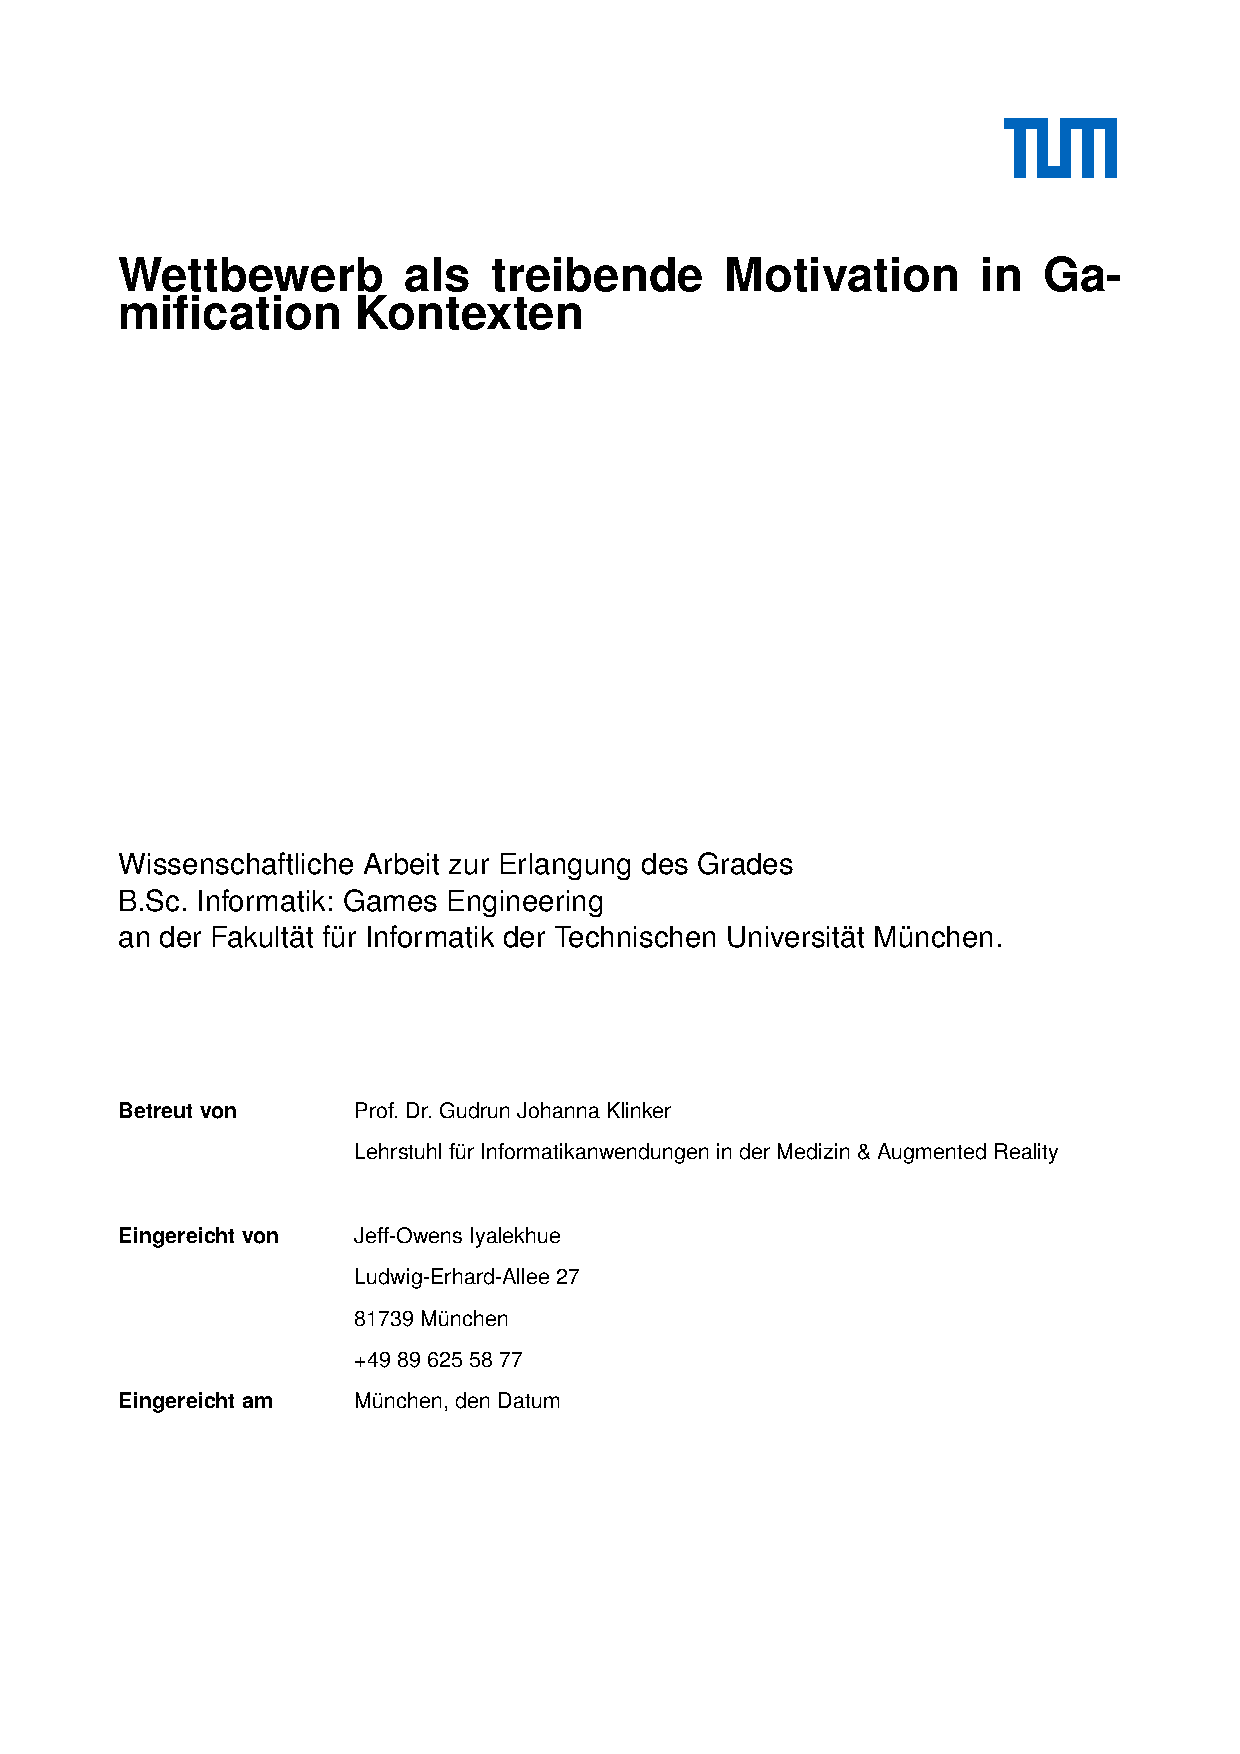
\includepdf[pages=-]{./Ressourcen/Deckblatt.pdf}
\tableofcontents % Inhaltsverzeichnis

\chapter{Abstrakt}

\chapter{Einleitung}
\section{Motivation}
Um Software neu und interessant zu gestalten wird Gamification oft als ein Designmethode verwendet. Die Effektivität dieses Vorgehens war deswegen bereits Subjekt einiger Studien. Diese Bezogen sich meist auf das jeweilige gewünschte Anwendungsgebiet, zum Beispiel ob ein Lerneffekt dadurch beeinflusst wird. In dieser Arbeit wird ein spezieller Aspekt aus spielerischen Kontexten betrachtet: Der Wettbewerb.\newline
Dies ist ein elementarer Teil vieler Spiele, aber auch in vielen anderen Kontexten ist er enthalten. Er ist eine Quelle der Motivation für Tätigkeiten, aber ob dieser Antrieb auch eine Wirkung auf die Ausübung
%neu formulieren
hat steht für uns noch offen. Daher wird der Einfluss von Wettbewerb auf die Leistung einer Person wird in dieser Thesis untersucht, dies speziell in einer spielerischen Umgebung. Auch ob die Motivation andere Auswirkung auf den Umgang mit dem Subjekt haben.
%
\section{Definitionen}
\subsection{Gamification}
Gamification beschreibt den Vorgang Komponenten, welche für Computerspiele charakteristisch sind, zu einer anderen Anwendung hinzu zu fügen. Dies soll der Verbesserung der modifizierten Anwendung. So soll das Interesse der Nutzer dadurch gesteigert oder ein Lerneffekt erhöht werden.

\subsection{Wettbewerb und Motivation}
Wettbewerb lässt sich als das Vergleichen von Leistungen definieren. Motivation lässt sich zwei Arten unterscheiden: intrinsiche und extrinsische Motivation.%\newline
Der intrinsische Motivation entspringt einem inneren Antrieb seine eigenen Fähigkeiten zu bestätigen.%\newline
Im Gegensatz dazu steht die extrinsische Motivation, bei der der Anreiz von einem äußeren Faktor entspringt. Im Fall eines Wettbewerb wäre der Anreiz üblicherweise der Sieg und damit das Besiegen des Gegenübers.\cite{Deci1981}




\chapter{Ansatz und Vorgehensweise}
 Um den Einfluss von Wettbewerb in der Leistung innerhalb eines spielerischen Szenarios beobachten zu können, braucht man eine Umgebung, in welcher dies unter verschiedenen Gesichtspunkten, möglich ist. Für diesen Zweck implementiere ich ein simples Computerspiel, mit dem die kognitiven Fähigkeiten einer Person testen, die Schwankungen in der Leistung aufzeichnen und verschiedene Testszenarien überprüfen kann. Zudem sollen die Teilnehmer der Testgruppen einen Fragebogen ausfüllen, der die Beobachtungen der Spielsituationen in einen Kontext setzt.
 
\section{Implementation}
Die Implementation kann in drei Bestandteile untergliedert werden. Im ersten Teil wird das Spiel entwickelt, mit dem später die Studie durchgeführt werden soll. Um zu überprüfen, ob dies wie erwartet funktioniert, wird eine Vorstudie durchgeführt. Anhand der Vorstudie sollen Fehler im Spiel behoben werden und erste Ansätze für die folgenden Beobachtungen in der Studie gefunden werden. Der letzte  Teil ist schließlich die Erkenntnisse der Vorstudie umzusetzen und die Testumgebung für die Studie vorzubereiten.

\subsection{Technologie}
Für die Entwicklung wird die Unity Engine 2018.2.2f1 verwendet. Diese Entwicklungsumgebung für Spiele bietet einige Grundlagen und Vorlagen, welche sich anbieten, da eine eigene Entwicklung einer Engine nicht Zielführend für die Arbeit ist. Für die Analyse der Dateien wird Microsoft Excel verwendet. Um die Fragebögen zu erstellen wurde der Dienst ''Google Formulare'' verwendet.

\subsection{Quellcode Zusammenfassung}
Die verwendete Programmiersprache ist C\#. In der Verwendung mit der Unity Engine wird auch dazugehörige Namespaces verwendet die wichtige Klassen und Funktionen zum erstellen eines Spiels anbieten. Die wichtigsten, selbst erstellten C\#-Skripte werden im folgenden zusammengefasst und ihr Nutzen beschrieben.
\subsubsection{GameManager.cs}
Diese Klasse verwaltet das Spiel mit den dazugehörigen Menüs.
\subsubsection{GameLogic.cs}
Diese Klasse beinhaltet die Logik des Mathe Spiels.
\subsubsection{MenuScript.cs}
Hier werden die Funktionen des Menüs zur Verfügung gestellt.
\subsubsection{NetworkMenu.cs}
Hiermit wird die Netzwerkverbindung erstellt und verwaltet.
\subsubsection{NetworkSync.cs}
Eine Helferklasse mit der die Abläufe einer Netzwerkverbindung synchronisiert werden sollen.
\subsubsection{NetworkObject.cs}
Die Repräsentation eines Clients im Spiel.

\subsection{Spielablauf}
In diesem Abschnitt wird der Ablauf ab Beginn des Programms beschrieben. Die Oberflächen bestehen aus Knöpfen und Eingabefeldern, navigiert und interagiert wird mittels Maus und Tastatur. Der erste Bildschirm ist das Netzwerkmenü (Abbildung \ref{network}), in welchen man wählen kann ob man als Host spielen will oder als Client. Für den Fall, dass man als Client spielt kann man in die Netzwerkadresse des Hosts und den dazugehörigen Port ändern.
\begin{wrapfigure}{r}{0.3\textwidth}
	\centering
	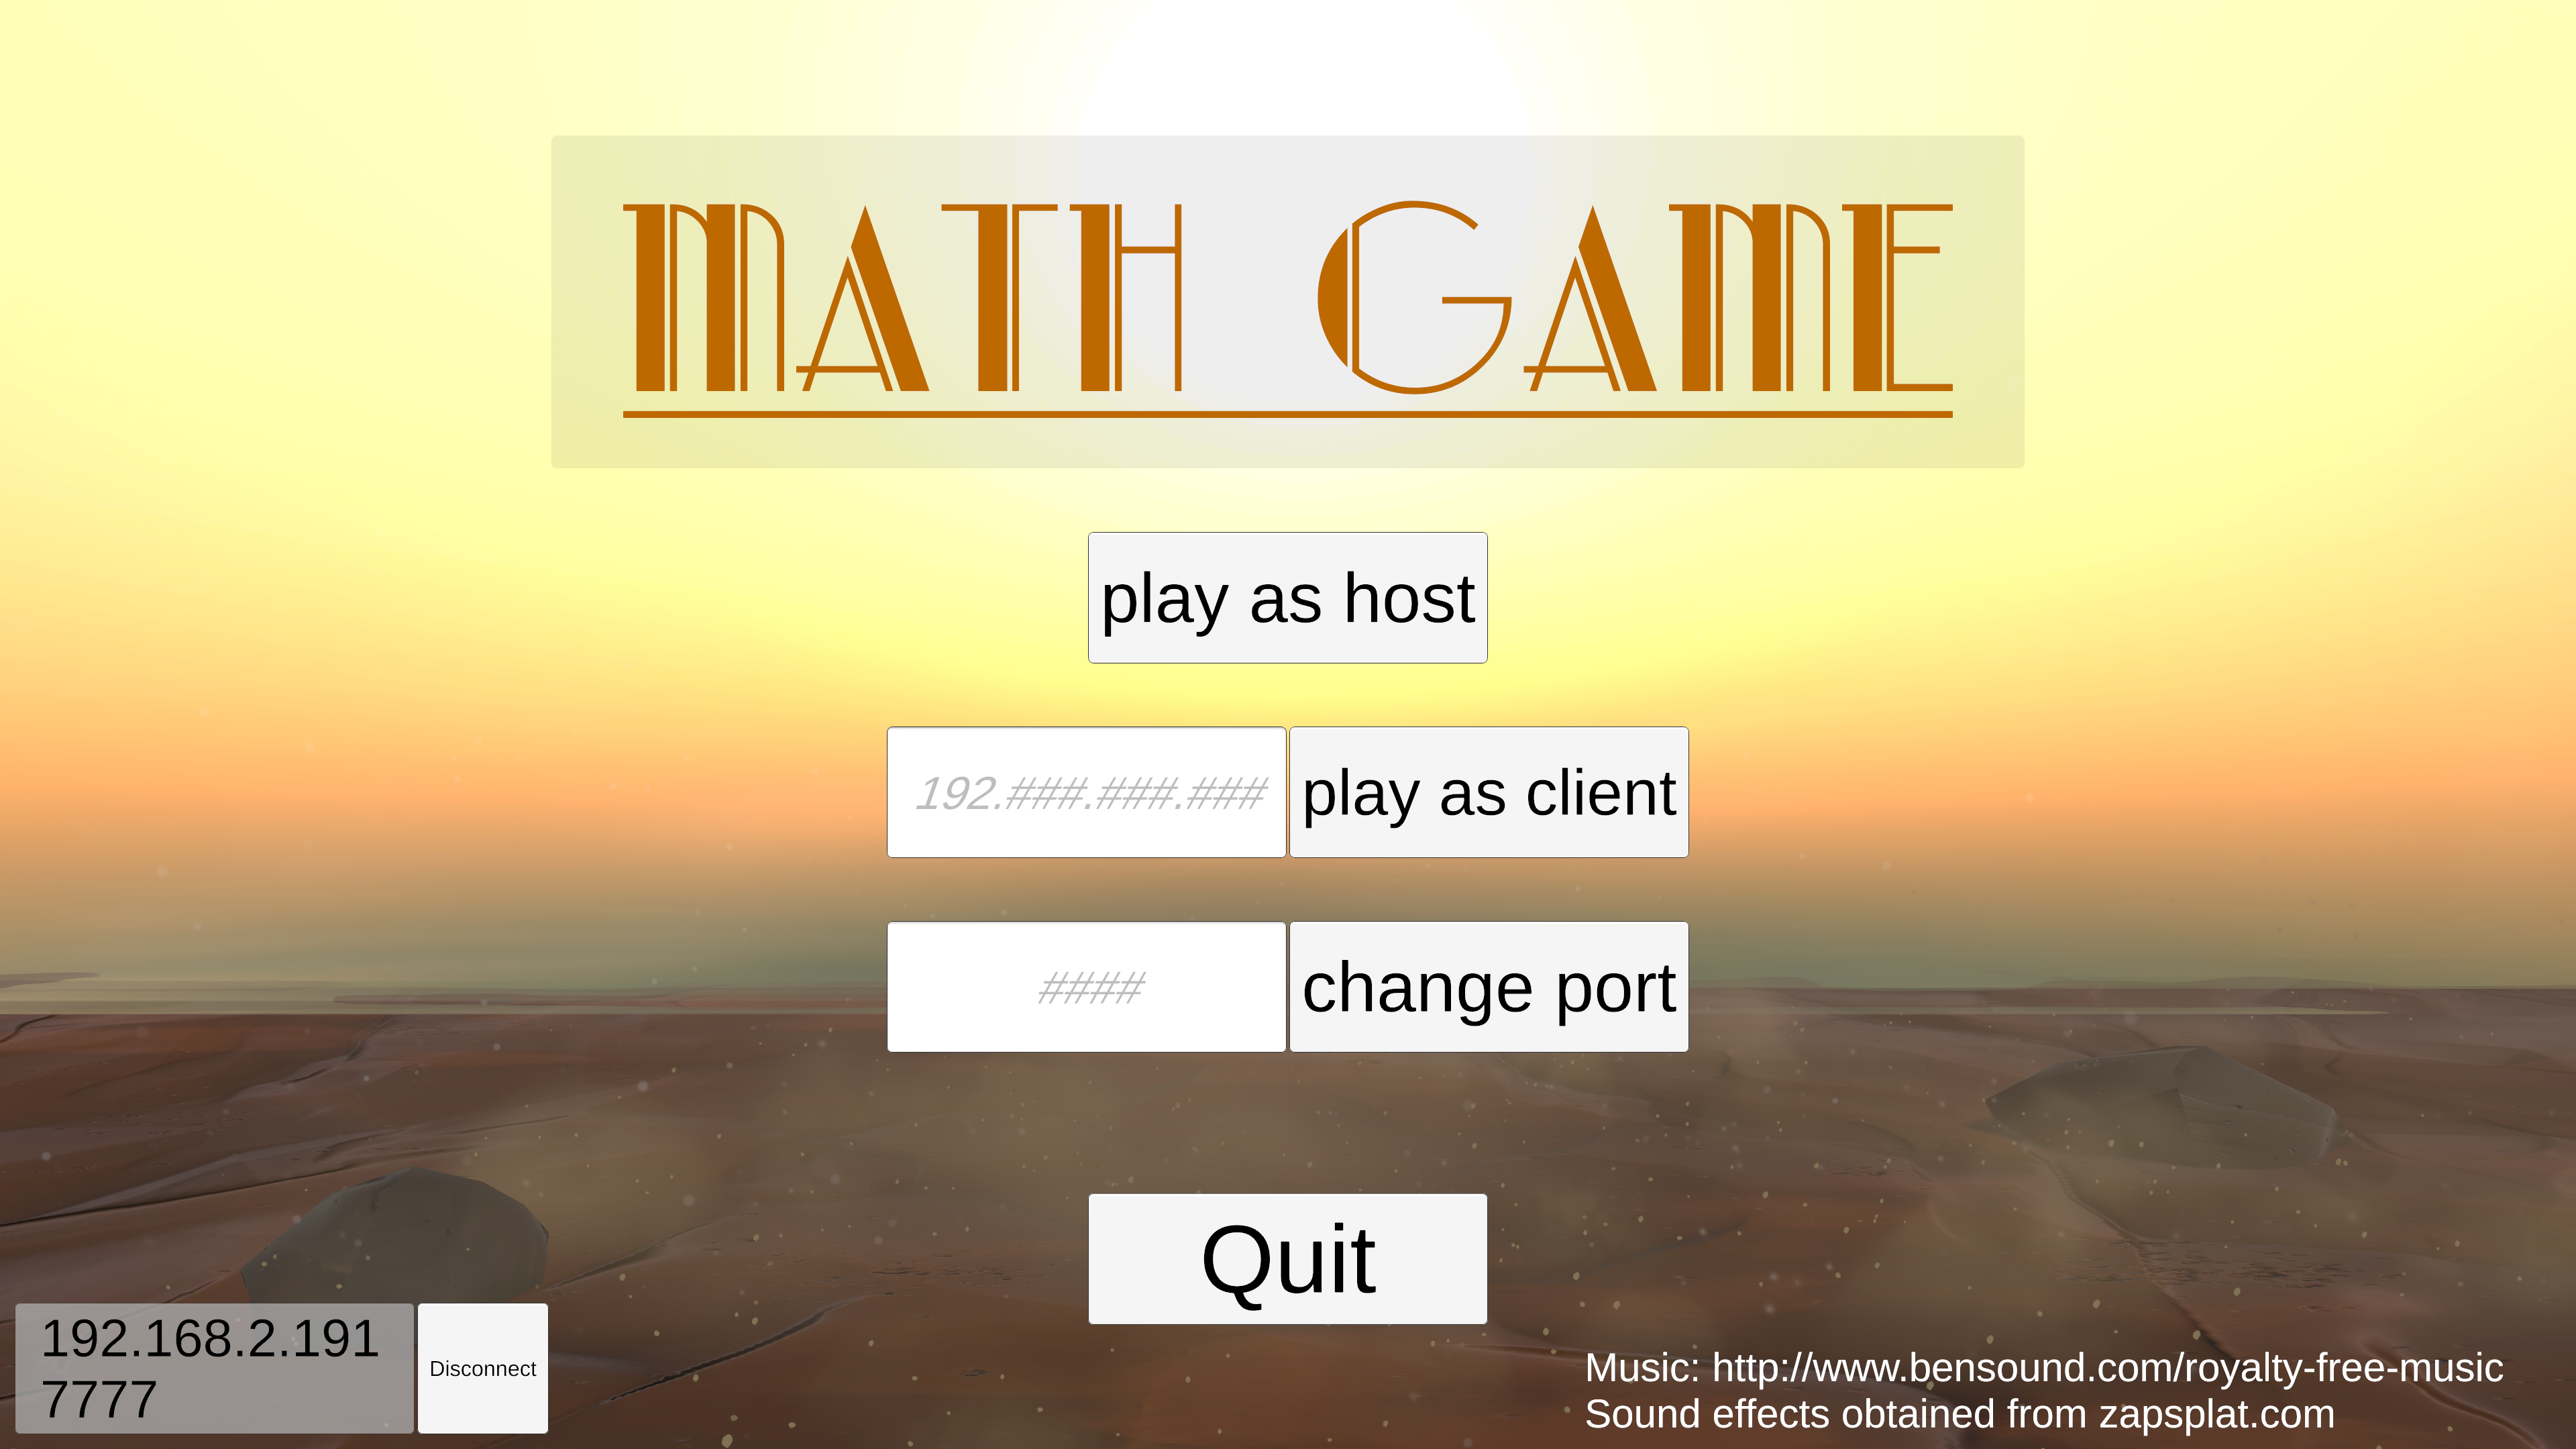
\includegraphics[width=0.3\textwidth]{networkmenu}
    \caption{Netwerkmenü}
    \label{network}
\end{wrapfigure}
\newline
Nach der Wahl zu hosten oder nicht wird man in das Hauptmenü weitergeleitet. Von hier aus kann man eine Runde des Spiels starten, wenn man Host ist den Spielmodus auswählen. in die Einstellungen wechseln, sich vom Netzwerk trennen und damit zurück in das Netzwerkmenü und die Software beenden.\newline
\begin{figure}[b]
	\centering
    \begin{subfigure}[a]{0.3\linewidth}
    	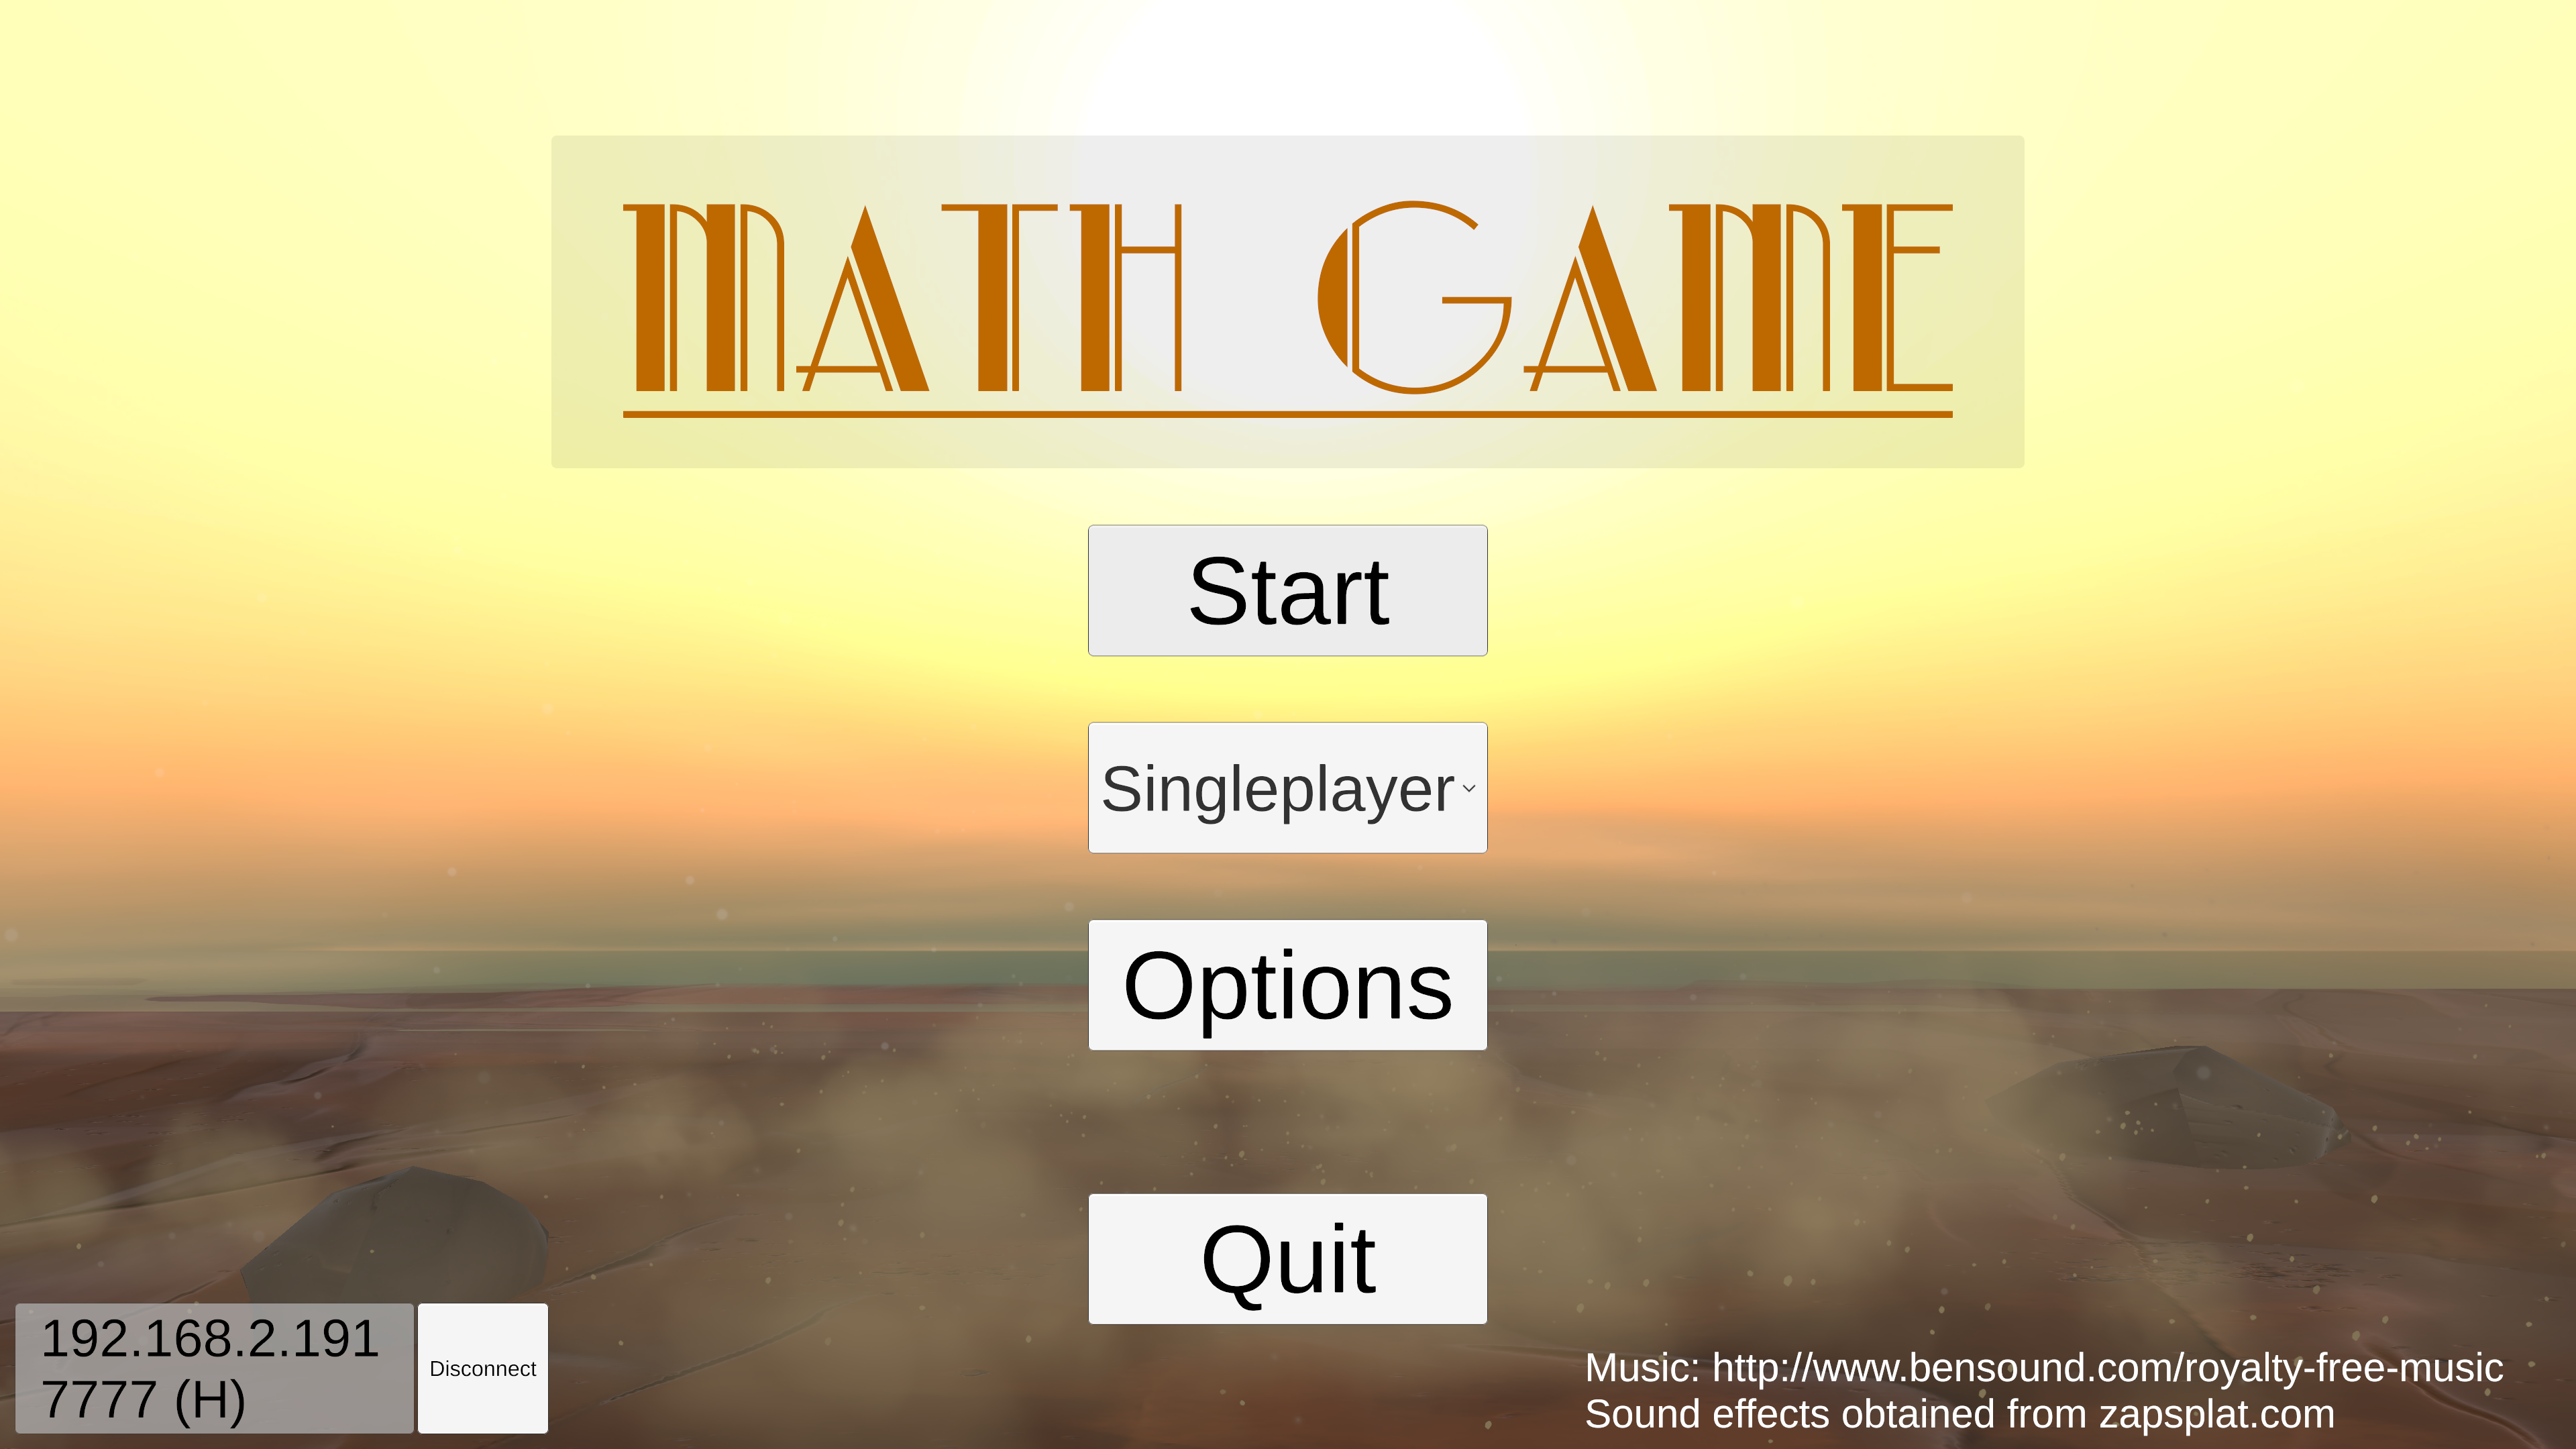
\includegraphics[width=\linewidth]{mainmenuhost}
    	\caption{Ansicht als Host}
        \label{fig:menuhost}
    \end{subfigure}
    \begin{subfigure}[a]{0.3\linewidth}
    	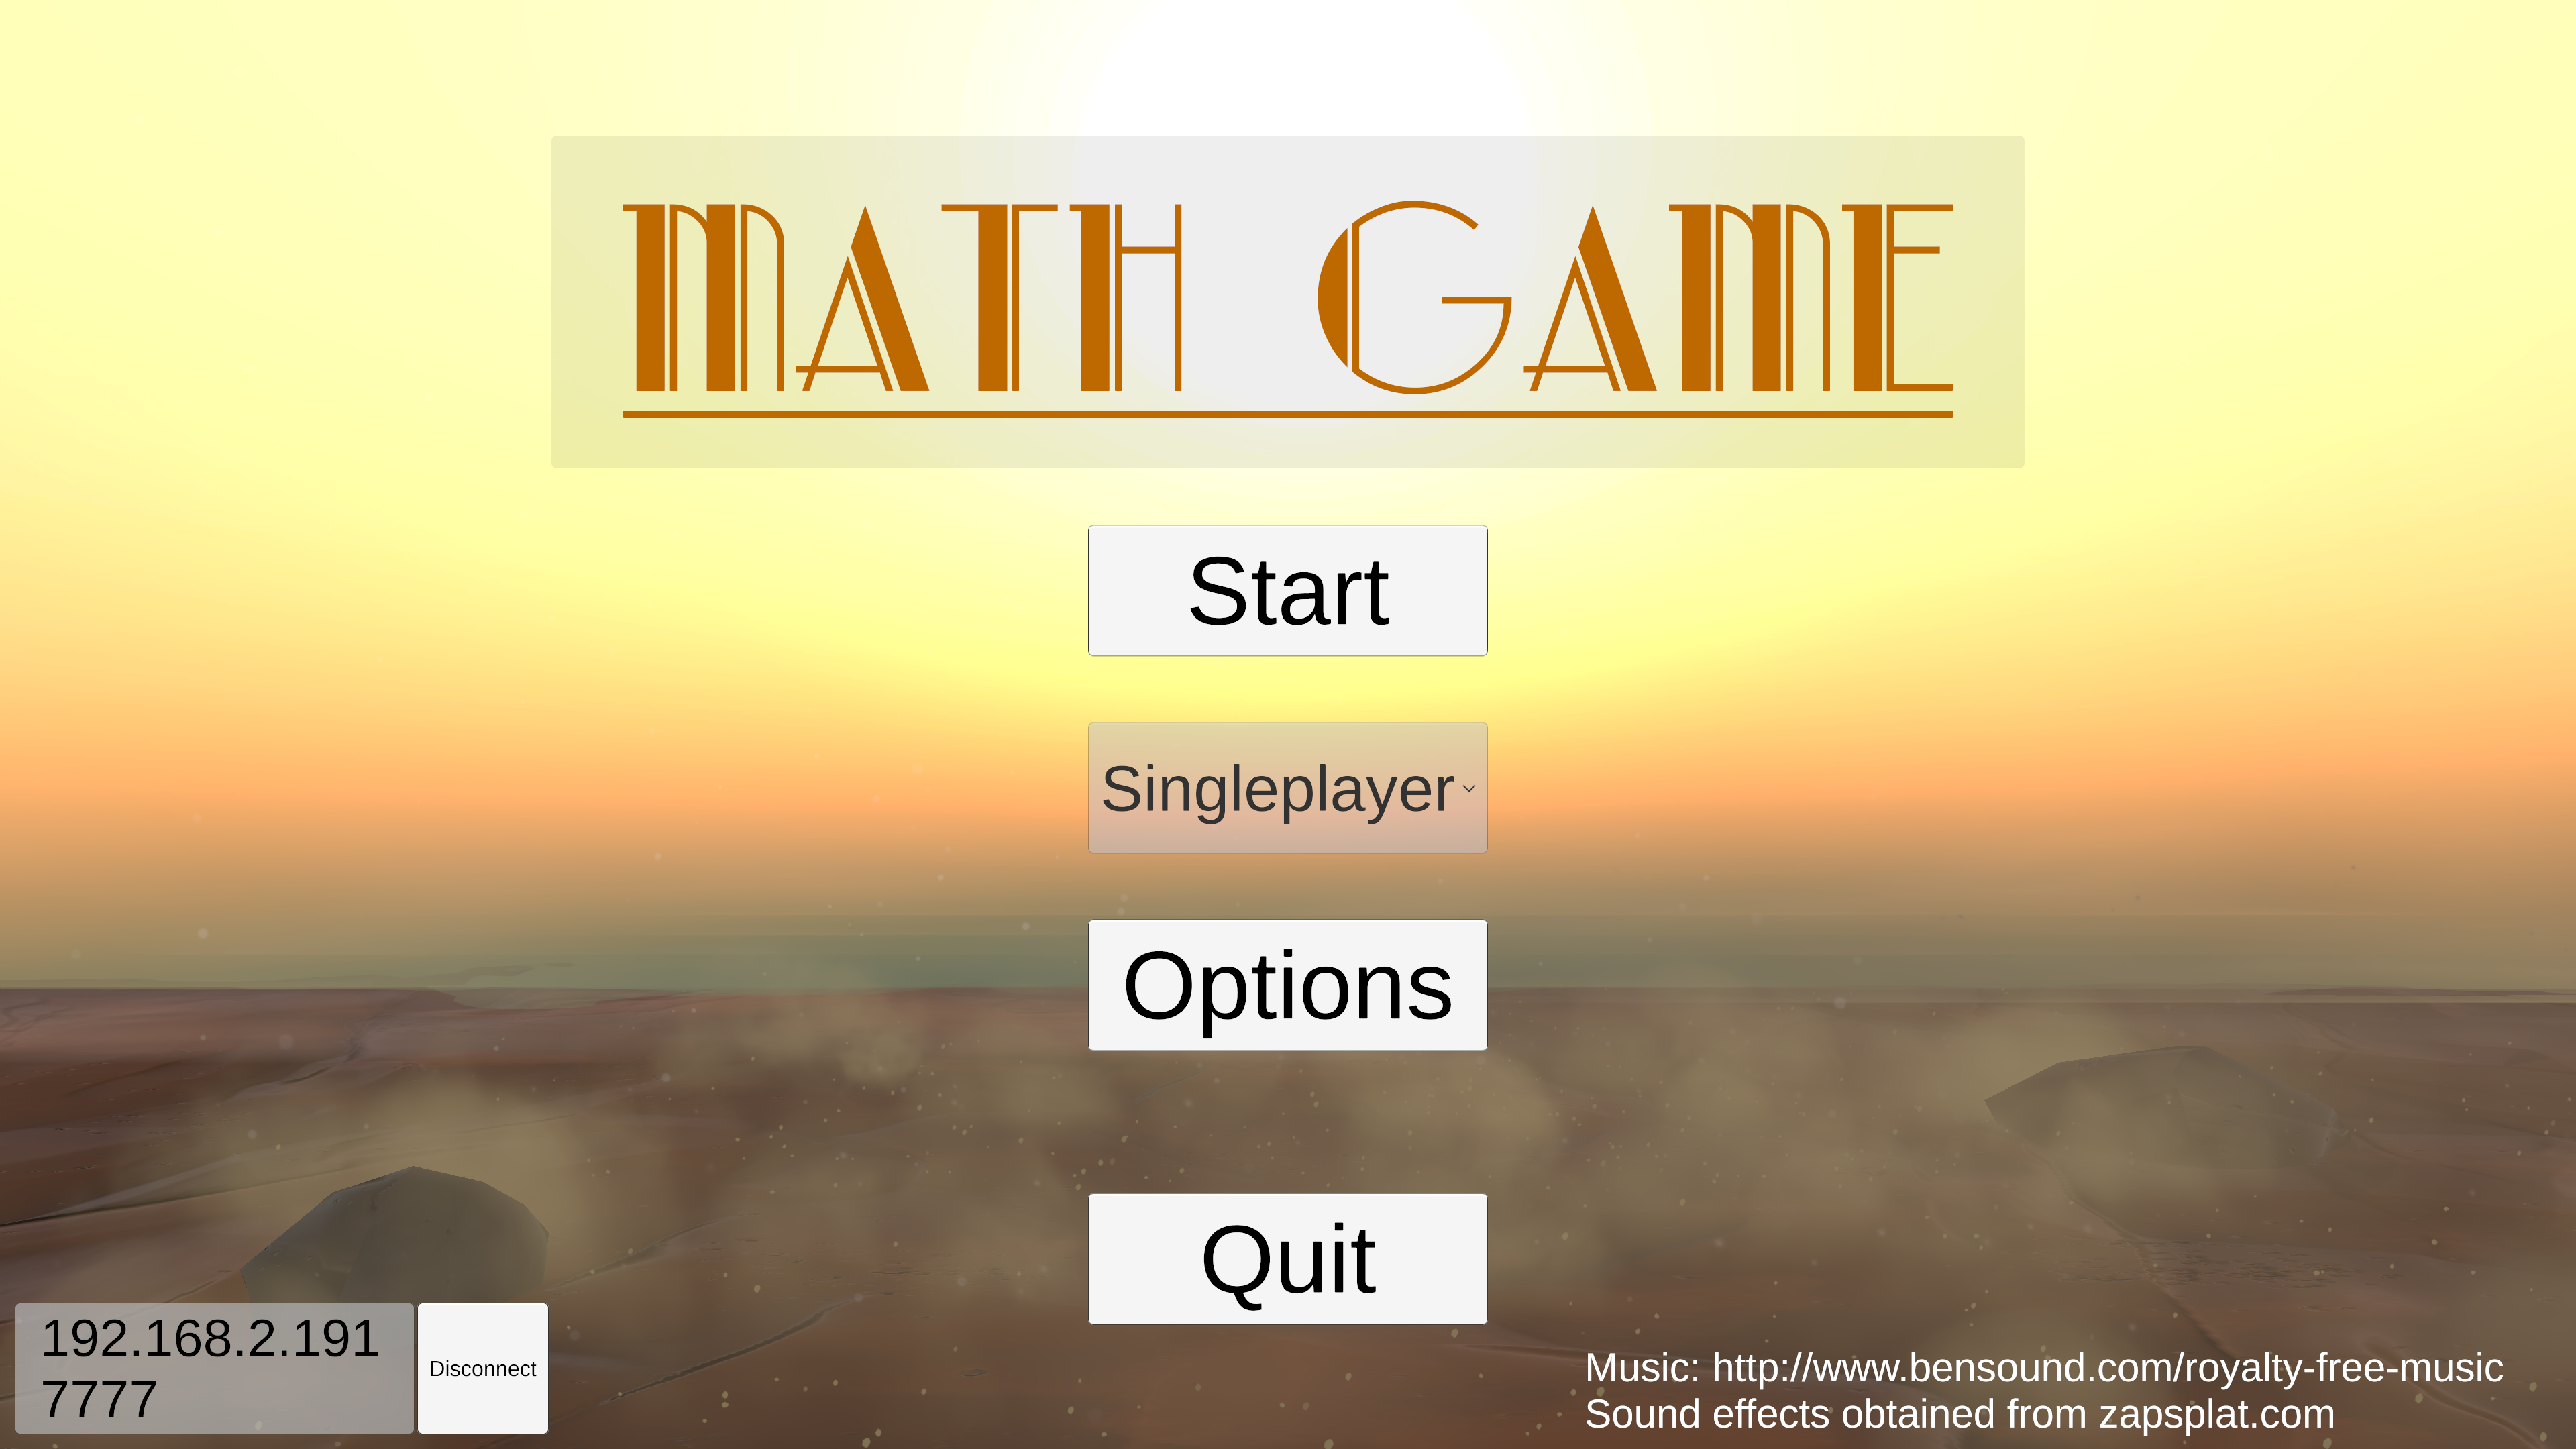
\includegraphics[width=\linewidth]{mainmenuclient}
    	\caption{Ansicht als Client}
        \label{fig:menuclient}
    \end{subfigure}
    \begin{subfigure}[a]{0.3\linewidth}
    	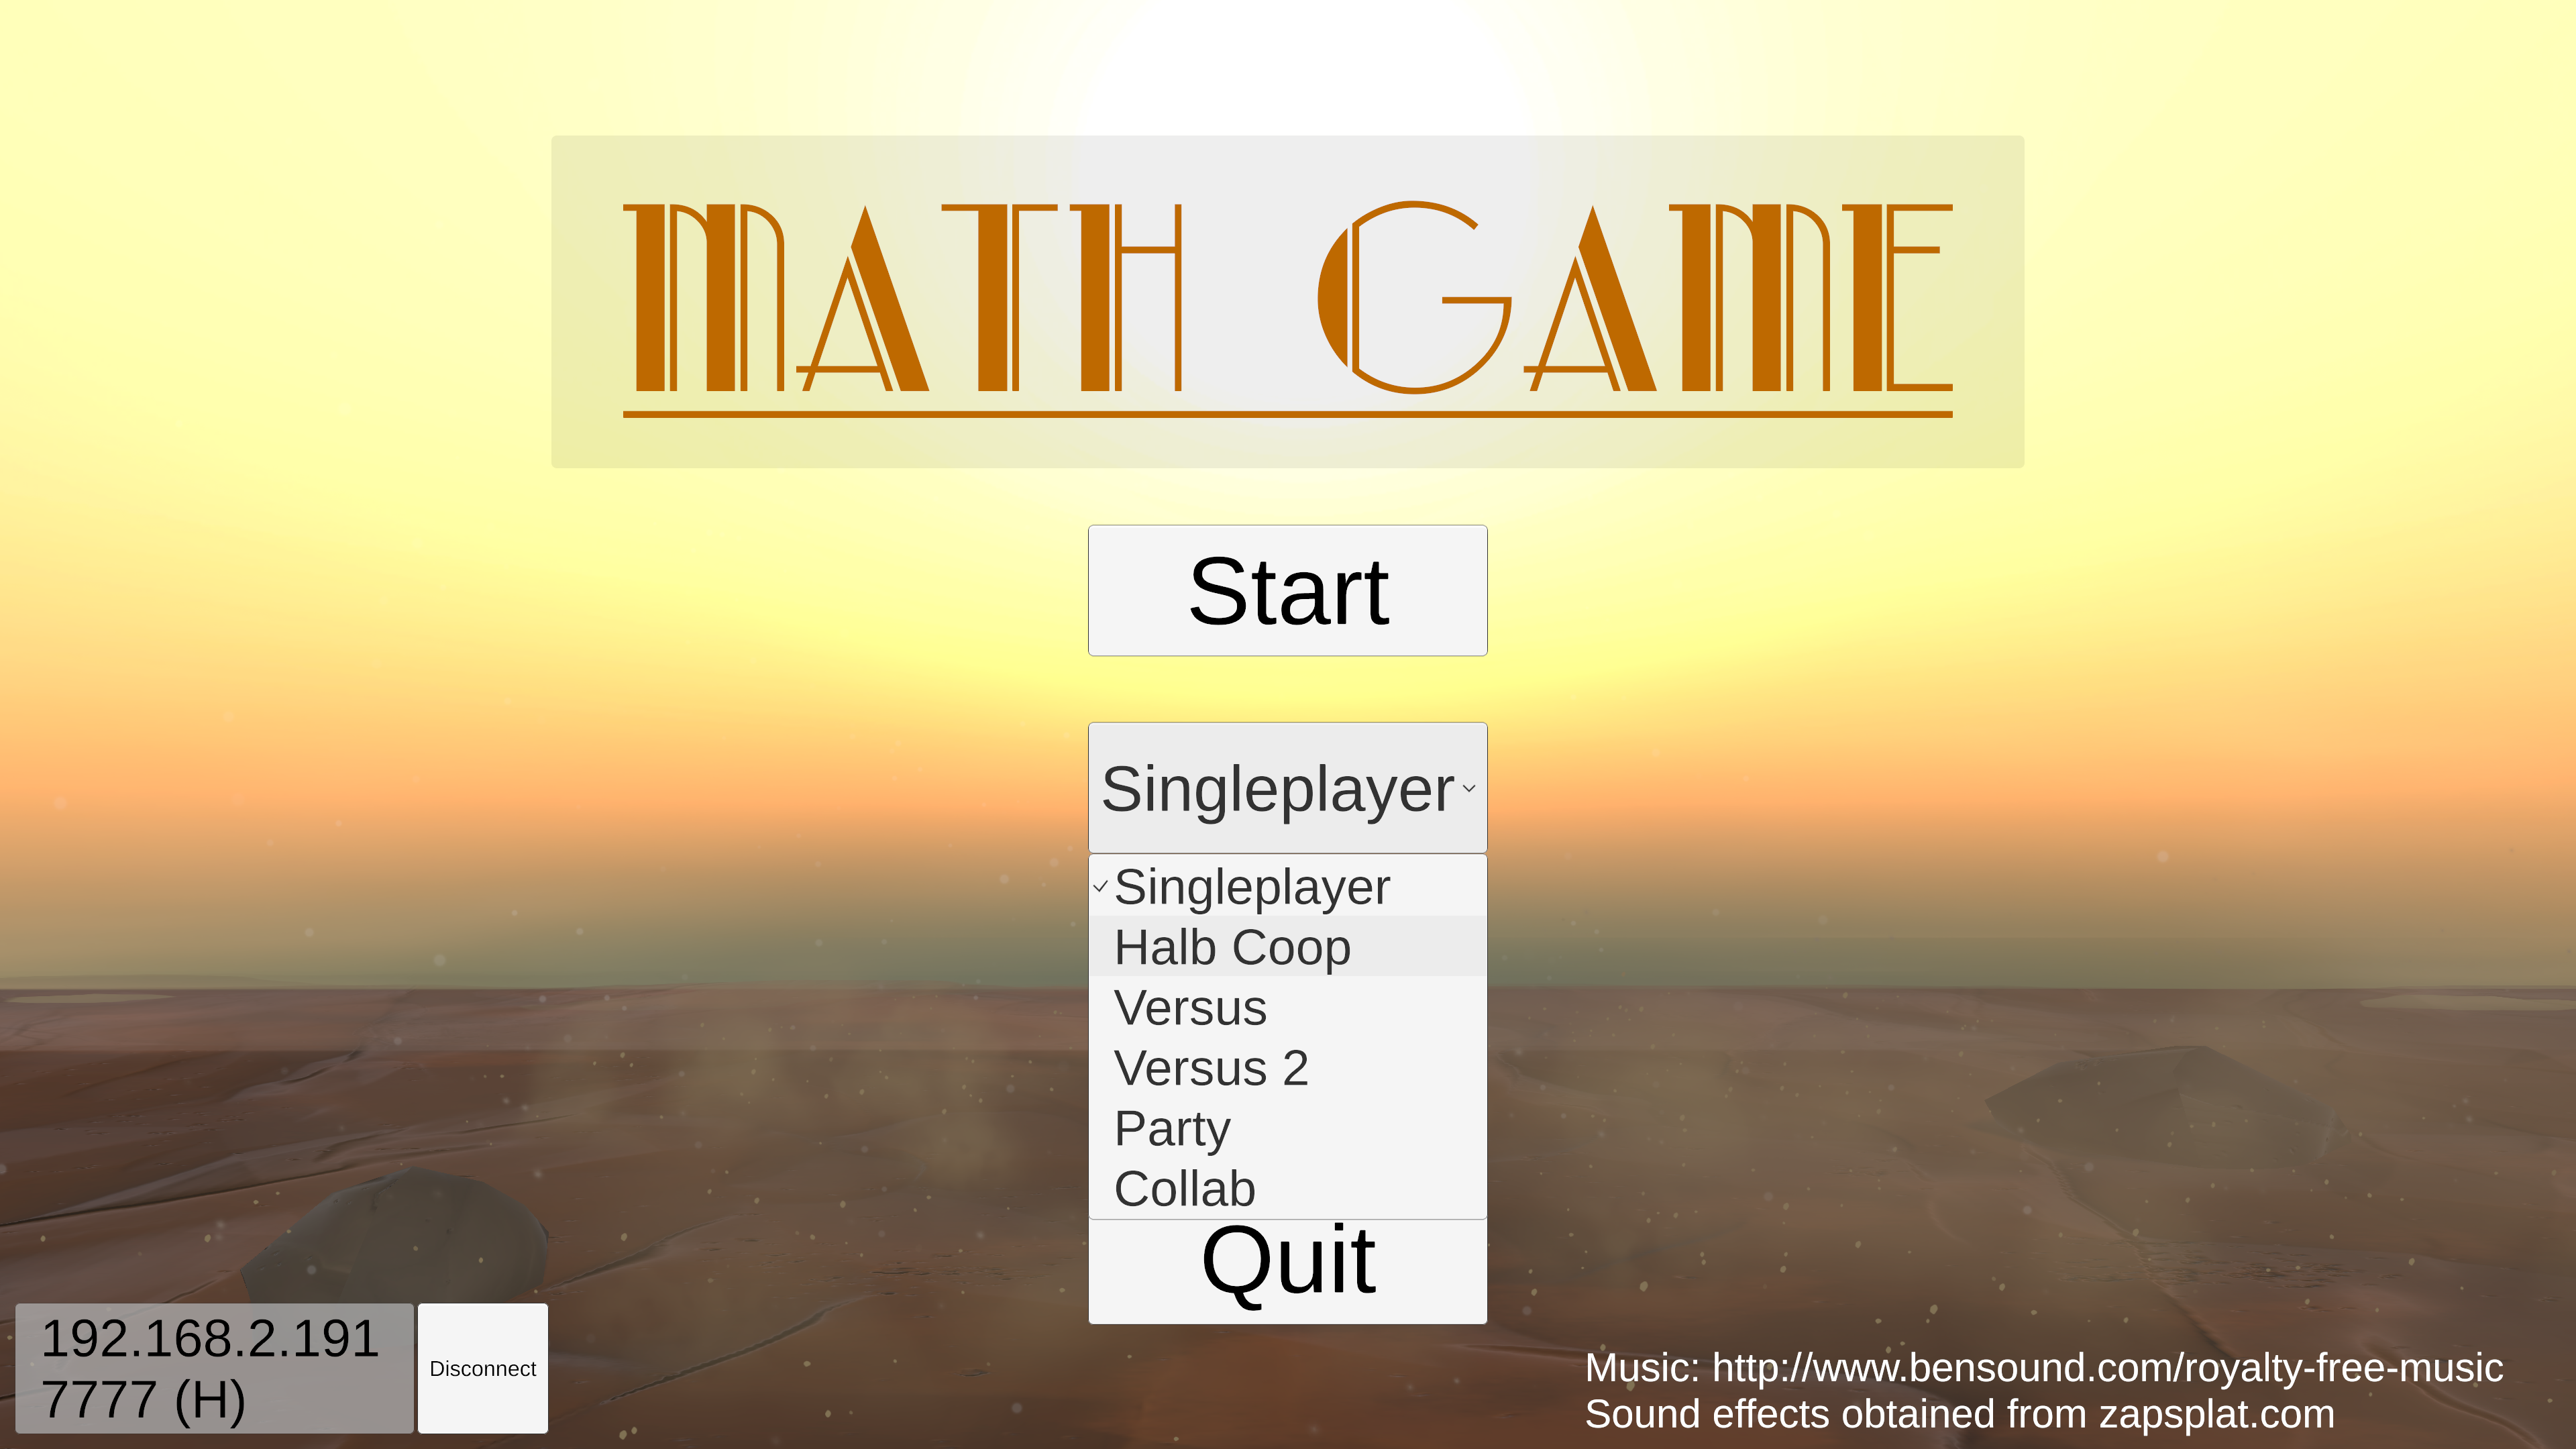
\includegraphics[width=\linewidth]{dropdownmenumodi}
    	\caption{Ansicht bei Wahl des Modus}
        \label{fig:menumodi}
    \end{subfigure}
    \caption{Ansichten des Hauptmenüs}
    \label{menu}
\end{figure}
In den Einstellungen kann man den Pfad angeben auf dem die Daten gespeichert werden sollen. Unter diesem Pfad werden die Logbuchdateien einer Spielrunde gespeichert, sowie die generierten Aufgaben. Wenn man Aufgaben erstellen will kann man hier sagen wie viele Funktionen pro Runde generiert werden sollen. Alternativ kann man auch einstellen, dass die Aufgaben während des Spielens zufällig erzeugt werden. Weitere Einstellungen beziehen sich auf die Darstellung des Spiels. So ist es möglich die Anzeigen für die verbleibende Zeit und die Punkte jeweils zu deaktivieren. Die Dauer einer Spielrunde wird auch hier bestimmt man kann, also angeben ob eine Runde nach einer gewünschten Zeit endet oder solange weiter geht bis der Nutzer sie per Tastendruck beendet. Auch die Lautstärke der Musik und der Soundeffekte lassen sich in den Einstellungen regulieren. Informationen zu dem Spieler die für die Logbuchdateien benötigt werden, werden auch hier angegeben, dazu zählt die Identifikationsnummer und das Geschlecht. Auch die Angabe in wie viele Runden bereits gespielt wurden lassen sich hier verändern. Wenn man die Einstellungen werden diese gespeichert, nur die Informationen zu einen Nutzer werden nicht persistent hinterlegt.\newline
Im Hauptmenü kann eine Spielpartie gestartet werden in dem auf den  ''Start''-Knopf gedrückt wird und alle nötigen Teilnehmer für den Modus bereit sind. Der ''Singleplayer''-Modus kann immer sofort starten, die anderen Modi verzögern den Spielstart bis alle mit dem Host verbundenen Spieler mit dem ''Start''-Knopf ihre Bereitschaft signalisiert haben. Während der Verzögerung können Nutzer durch erneutes betätigen des Knopfes die Bereitschaft wieder aufheben.\newline
Im Spiel hat man mehrere Anzeigen und ein Eingabefeld. Die folgende Oberfläche beschreibt einen generellen Fall des Spielmodus und trifft am ehesten auf den ''Singleplayer''-Modus zu. Die Anzeige am mittigen, oberen Bildschirmrand ist die verbleibende Zeit, darunter findet man die ''Score''-Einblendung. Zentral und im Verhältnis am größten dargestellt findet man die zu lösende Rechnung. Unterhalb der Aufgabe ist das Eingabefeld in dem die Lösung eingegeben wird. Zur Eingabe wird die Tastatur verwendet, wobei nur Zahlen eingeben und das '-'-Zeichen akzeptiert werden. Mit der ''Enter/Return''-Taste wird eine Eingabe bestätigt, mit der ''Backspace''-Taste können unbestätigte Eingaben wieder rückgängig gemacht werden. Wenn eine Aufgabe richtig beantwortet bekommt man einen Punkt zum Score hinzu, dies wird durch einen Ton und einer Animation zusätzlich visualisiert. Für den Fall einer falschen Lösung wird die Punktzahl um einen Punkt reduziert, dass überspringen einer Aufgabe ist auch möglich wenn eine leere Eingabe bestätigt wird. Überspringen gibt keinen Punkt zum Score, zieht aber auch keinen ab. Auch das Verlieren oder überspringen einer Aufgabe hat jeweils eine eignen Animation und einen Ton.

\subsubsection{Modi und Testszenarien}
Das Spiel besitzt verschiedene Modi um die unterschiedlichen Testszenarien abzubilden. Die Modi erben in einer bestimmten von einem Standardmodus. Der Ursprungsmodus lässt sich schon mittels der Einstellungen modifizieren. Änderungen durch veränderte Einstellungen sind zum Beispiel die Dauer des Spiels, das Anzeigen der erzielten Punkte oder der verbleibenden Zeit. Das Spiel terminiert entweder manuell nach dem betätigen der 'escape'-Taste oder nach einer gesetzten Zeit, da diese auch als 'unendlich' eingestellt werden kann, ist das händische Beenden immer möglich. Die Aufgaben können während eines Spieldurchlaufs zufällig generiert werden oder im Vorfeld erstellt, gespeichert und dann für ein Spiel geladen werden. Im folgenden werden alle implementierten Modi beschrieben:\itemize
\begin{figure}[b]
	\centering	
	\begin{subfigure}[a]{0.3\linewidth}
		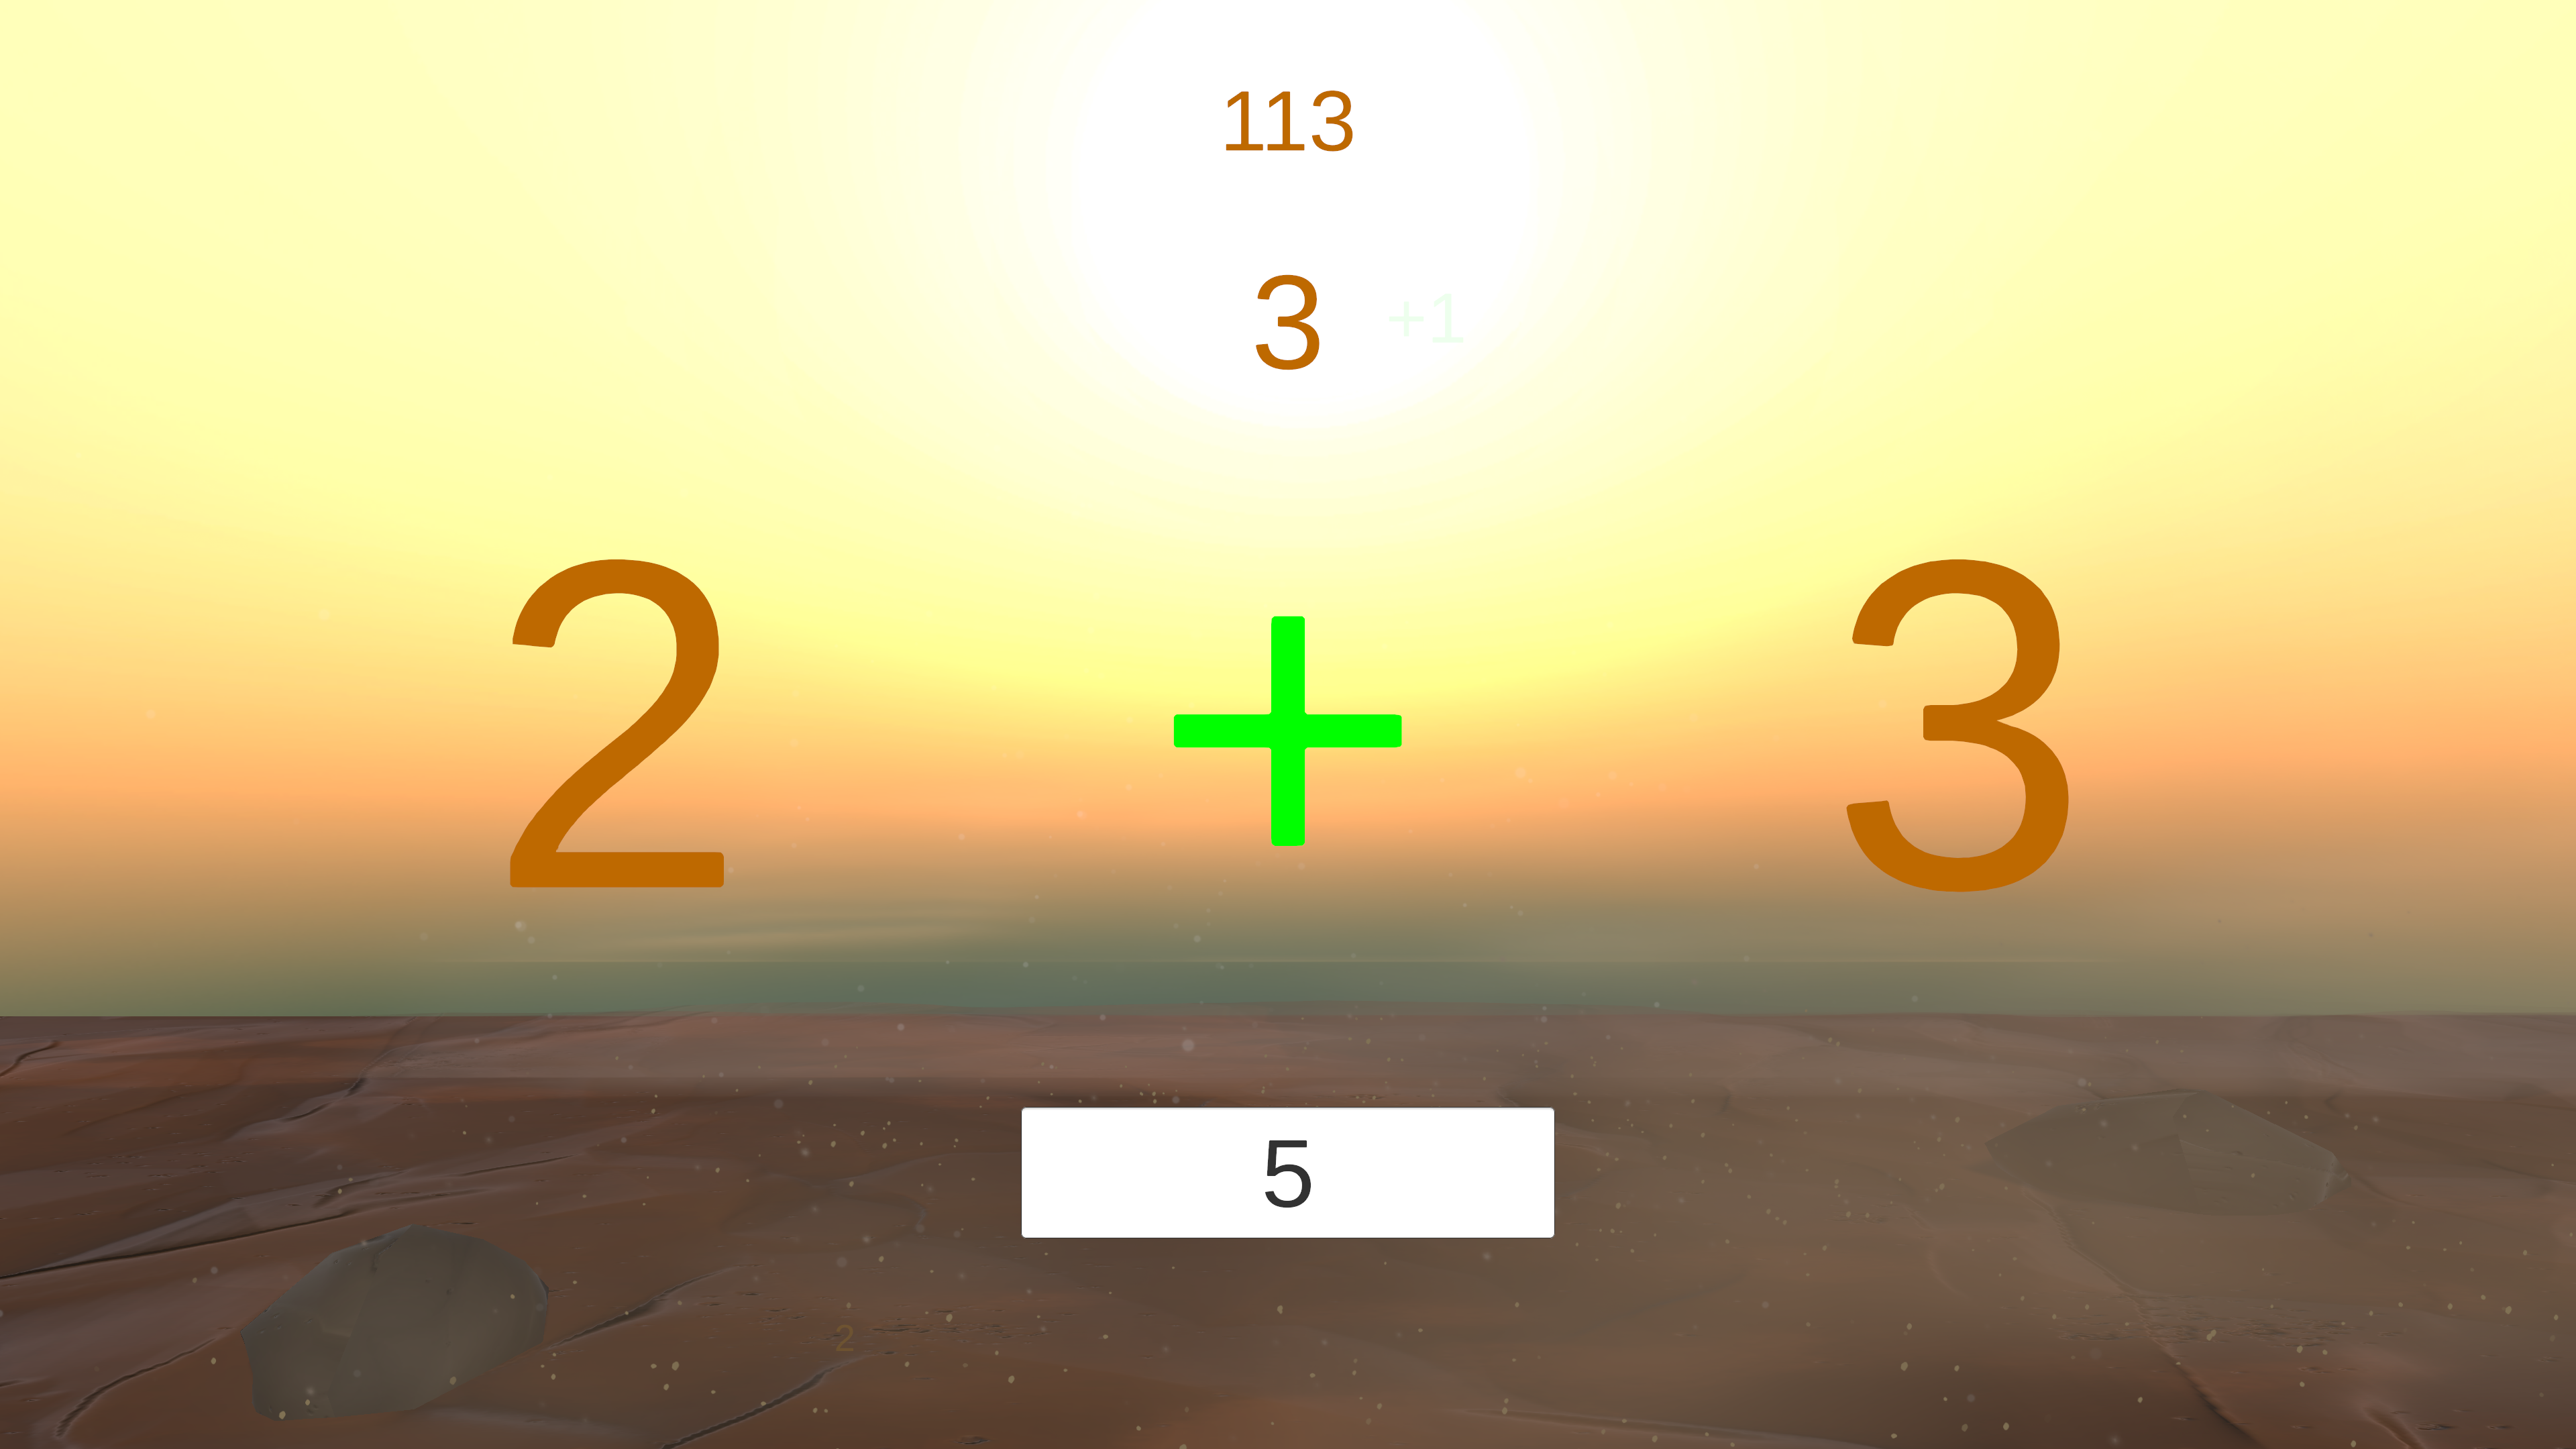
\includegraphics[width=(\linewidth)]{singleplayer}
		\caption{Singleplayer}
		\label{fig:singleplayer}
	\end{subfigure}	
	\begin{subfigure}[a]{0.3\linewidth}
		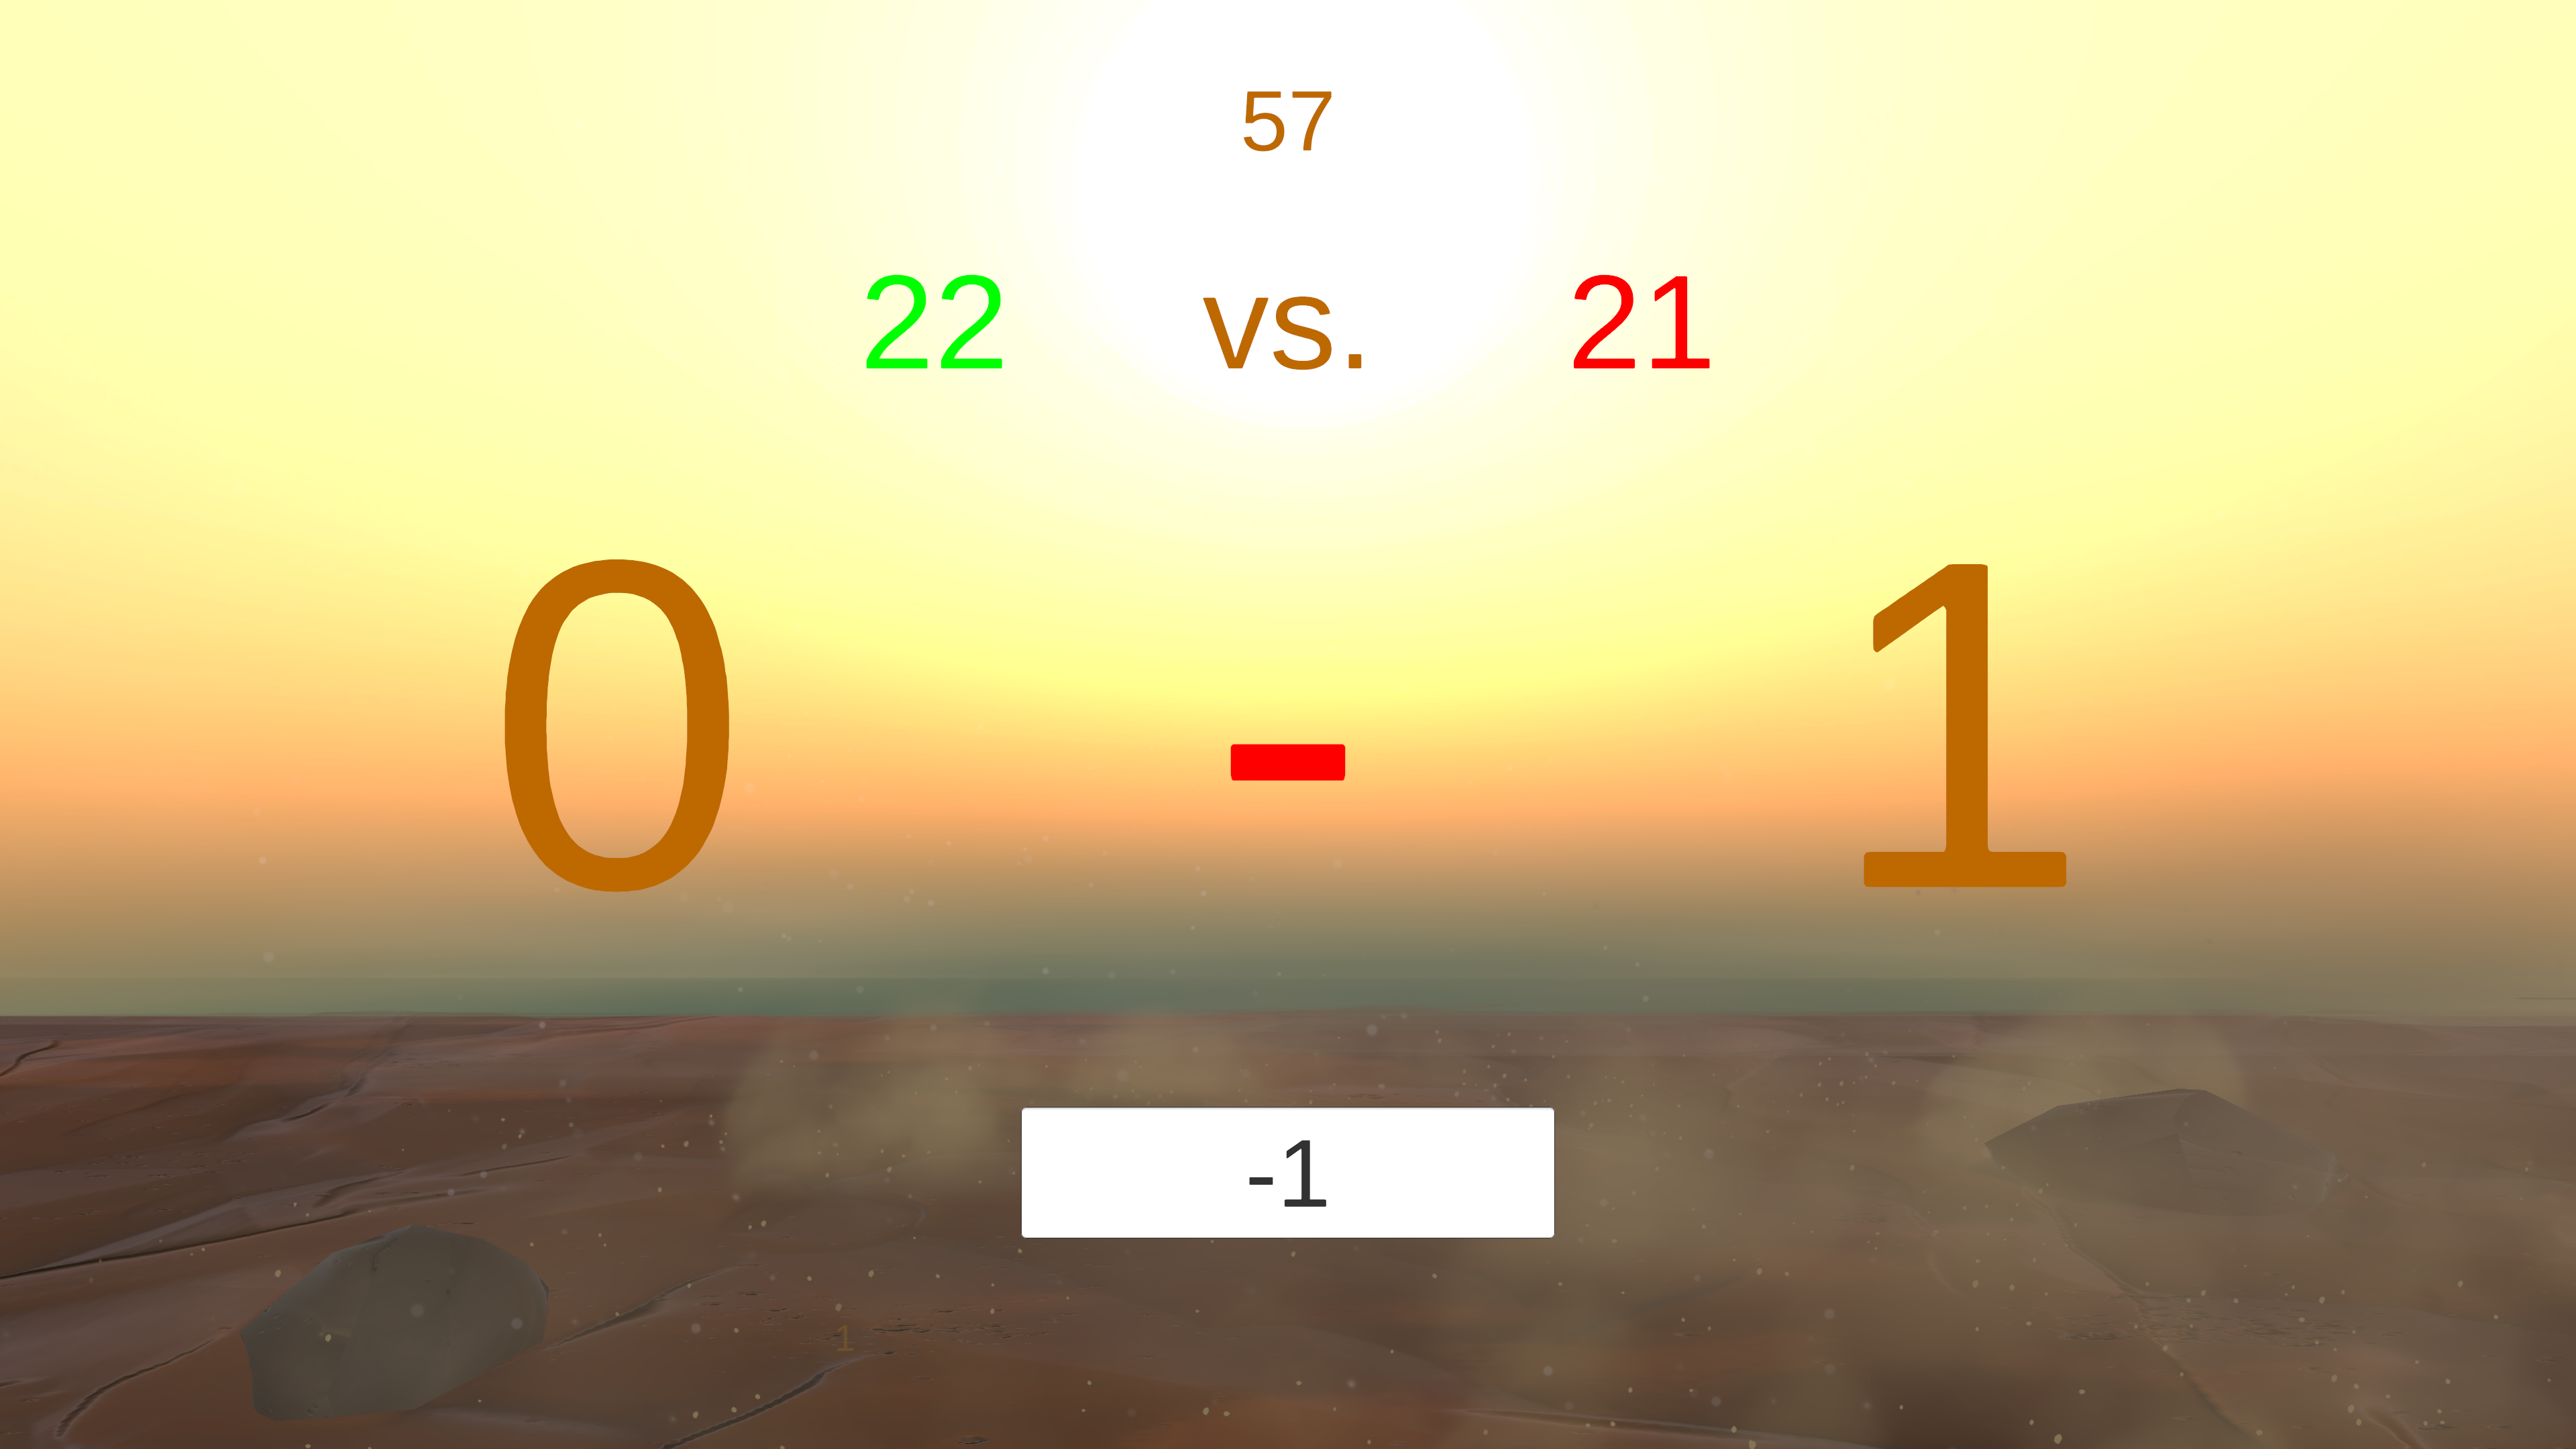
\includegraphics[width=(\linewidth)]{versus}
		\caption{Versus}
		\label{fig:versus}
	\end{subfigure}
	\begin{subfigure}[a]{0.3\linewidth}
		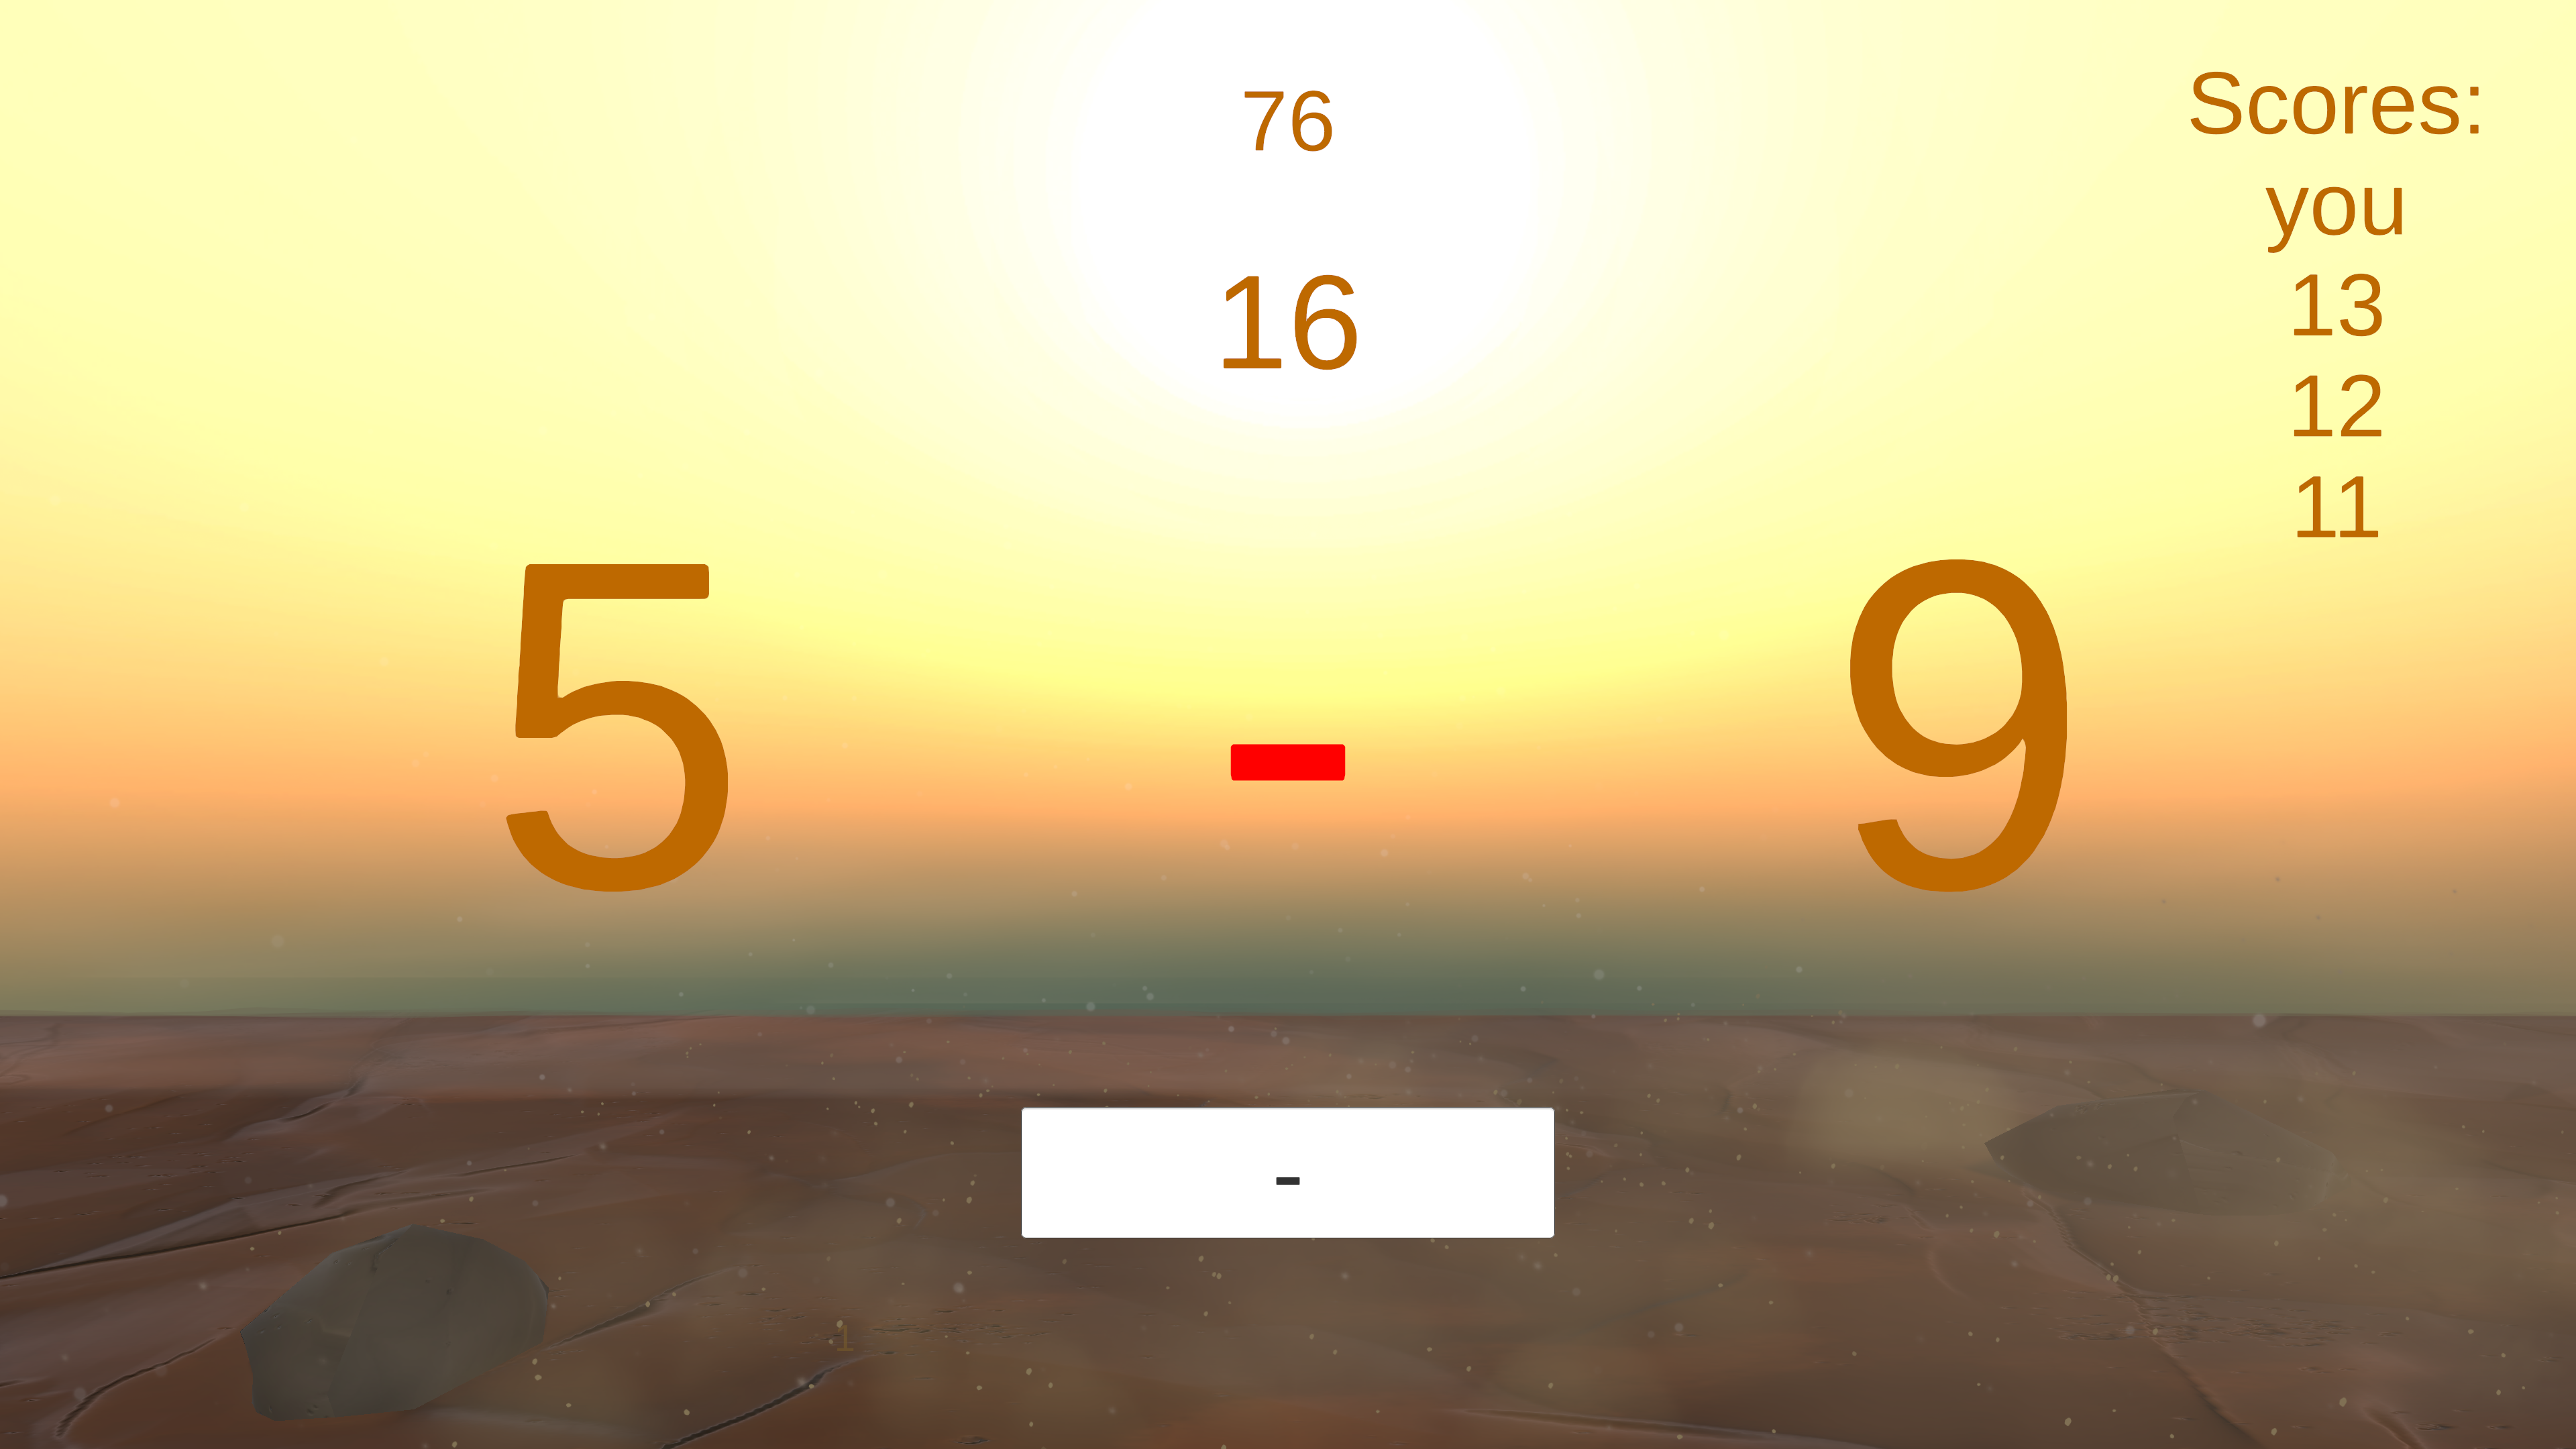
\includegraphics[width=(\linewidth)]{party}
		\caption{Party}
		\label{fig:party}
	\end{subfigure}	
	\caption{Bildschrimaufnahme der Modi}
    \label{fig:modi}
\end{figure}

\item''Singleplayer''-Modus:\newline
Dieser Modus entspricht dem Basisspiel. Man spielt ohne Gegner und versucht einen möglichst hohe Punktzahl zu erzielen. Die Anzeige auf dem Bildschirm entsprechen der Abbildung \ref{fig:singleplayer}.
\item''Halb-Coop''-Modus:\newline{}
Der Gedanke in dieser Variante ist das zwei oder mehrere Menschen den Einzelspielermodus parallel spielen. Dafür synchronisiert sich der Start des Spiels der Personen. Ansonsten entspricht alles dem Basisspiels. Das Erscheinungsbild entspricht dem ''Singleplayer''-Modus
\item''Versus''- \& ''Versus2''-Modus:\newline
Der ''Versus''-Modus entspricht einer klassischen Umsetzung von Wettbewerb, zwei Spieler spielen gegen einander. Die Punktzahlen von beiden werden gegenübergestellt, damit ein Vergleich der Leistung stattfinden kann. Die Punkteanzeige auf dem Bildschirm eines Nutzers ist in dieser Variante leicht modifiziert,  vergleiche Abbildung \ref{fig:versus}, denn sie zeigt  auch den Punktestand des Gegenübers an (Bsp. X vs. Y, mit X als die Punktzahl des Spielers und Y als die des Gegners). Die zwei Varianten unterscheiden sich nur im Namen, dies Unterteilung ist für die Logbuchdateien notwendig.
%\item''Versus 2''-Modus:\newline
\item''Party''-Modus:\newline
Um den Wettbewerb mit mehreren Teilnehmern darzustellen wurde dieser Modus implementiert. Die Teilnehmerzahl ist variabel und wird mit ''falschen Spielern'' von Spiel aufgefüllt, wenn eine gewünschte Spielerzahl nicht mit Nutzern erreicht wird. Das Userinterface ähnelt mehr dem der Einzelspielermodi als dem der ''Versus''-Modus, mit einem unterschied es gibt eine Ranglistenanzeige, die die Punkte der Nutzer und der, falls vorhanden, falschen Spieler in Verhältnis setzt. Die Person ganz oben in der Liste hat die höchste Punktzahl, wenn man nicht an dieser Position ist signalisiert die Liste das, indem sie leicht pulsiert. Abbildung \ref{fig:party} zeigt eine Bildschirmaufnahme dieses Modus.
\item''Collab''-Modus:\newline
Ein Modus, der etwas gegen den Gedanken der anderen Modi geht, wurde auch implementiert.  In diesem Modus kooperieren die Spieler um einen gemeinsamen Punktstand zu erhöhen. In diesem Modus entspricht der Bildschirm wieder dem des Basisspiels, der unterschied zwischen einem eigen Beitrag zum Punktestand und dem eines Mitspielers, ist die Animation ob man einen oder keinen Punkt hinzugefügt, beziehungsweise abgezogen hat. Ähnlich wie der ''Halb-Coop''-Modus entspricht die Anzeigeart der des ''Singleplayer''-Modus.
%further improvement of visual (on going)\newline
%usability improvements

\subsubsection{Datensammlung und Spielverlaufslogbuch}
Während eines Spieldurchlaufs wollen wir verschiedene Faktoren beobachten, um Rückschlüsse auf die Einflüsse der Testszenarien  machen zu können. Für diesen Zweck sammeln wir  Daten des Spielverlaufs und lassen sie uns für eine spätere Analyse speichern. Vom Spiel werden nach einer Runde drei Dateien angelegt, die die gewünschten Ereignisse dokumentieren. Die Logbuchdateien eines Spielers werden in einen Ordner unter einem angegeben Pfad gespeichert, welcher in der Form ''ParticipantX'', wobei X der jeweiligen Nutzeridentifikationsnummer entspricht (Bsp. Participant1), benannt wird. Die drei Dateien einer Runde Unterscheiden sich im Dateiformat und gering  im Informationsgehalt. Die im Spiel zu beobachteten Variablen werden zum einen serialisiert und dann als ''.dat'' gespeichert, diese Dateien dienen ausschließlich als redundante Sicherheitskopie und könnten wieder deserialisiert und  geladen werden. Dies ist im Code nicht umgesetzt worden, da keine Notwendigkeit bestand.\newline
Um den Verlauf einer Runde in der Retrospektive nachvollziehen zu können, werden als ''.txt''-Dateien stichpunktartige Protokolle der Ereignisse dokumentiert.\newline
Für die Datenauswertung  werden hauptsächlich die ''.csv''-Dateien verwendet. Solche Dateien können in Programmen, die speziell für die Datenverarbeitung  und Analyse dienen, eingelesen und verarbeitet werden.
%bug fixes\newline
%removal of animations\newline
%scripted player\newline
\subsection{Vorstudie}
Mit der Vorstudie wurde die Lauffähigkeit des Spiels getestet und versucht einen ersten Ansatz für mögliche Beobachtungen in der Haupttestreihe zu finden. Es wurden die Modi ''Singlepayer'', ''Halb-Coop'', ''Versus'' und '' Party'' von fünf Teilnehmern gespielt. Anhand der Impressionen wurden Fehler im Spiel ausgebessert und Änderungen vorgenommen, so wurden die Eingangs- und Austrittsanimationen der Aufgaben entfernt damit ein ununterbrochener Spielablauf entstehen kann. Auch die Wahl der zu testenden Modi wurde geändert. Die nun in der Hauptstudie zu Testenden Szenarien sind  ''Singleplayer'', ''Halb-Coop'', ''Versus'' und ''Versus2''.

%first data impression (no learning in later turns?)
%bug report
\subsection{Fragebogen}
Neben der reinen Beobachtung des Spielverlaufs sind auch Ausagen und Eindrücke der Spieler nützlich um Daten in Kontexte zu stellen und zu Interpretieren. Hierfür eignet sich die Beantwortung eines Fragebogens durch die Teilnehmer.
%bug fixes\newline
%removal of animation

\section{Aufbau}
Für einen Durchlauf wird ein einzelner Teilnehmer in den Versuchsaufbau gebeten. Es sind zwei Computer aufgebaut auf denen das Spiel läuft und die über das Netzwerk miteinander verbunden sind. Zunächst füllt er den ersten Teil des Fragebogen aus. Anschließend spielt er einen Modus und beantwortet danach den zugehörigen Teil des Fragebogens. Dies wiederholt er bis er alle Modi gespielt hat. Die Reihenfolge der Modi für jeden Teilnehmer durch, sodass erst bei mehr als 24 Teilnehmern die Reihenfolge sich wiederholt. Zwischen den Spielszenarien lassen sich drei verschieden Aufbauten definieren, die alle die gemein haben, dass die Versuchsperson nicht alleine sondern immer unter Aufsicht des Betreuers ist. Beim ''Singleplayer''-Modus spielt der  Teilnehmer alleine und wird vom Versuchsleiter nur beobachtet. Der ''Halb-Coop''-Modus  versucht einen indirekten Wettbewerb aufzubauen in dem der Spieler zeitgleich mit dem Betreuer den ''Singleplayer''-Modus spielt und zusätzlich die Möglichkeit bekommt den Bildschirm des Gegenübers zu sehen. Allerdings wird ihm dieses Szenario als eine Variante beschrieben wo er nur auf sein Spiel achten braucht. Im Gegensatz dazu wird in den Modi ''Versus'' und ''Versus2'' direkt auf den Vergleich der Punktzahlen hingewiesen. In diesen Varianten sieht der Spieler nur seinen eigenen Bildschirm und bekommt daher nur über den Anzeigen in seinem Spiel den Fortschritt seines Gegenspieler mit. Der Unterschied der beiden Szenarien ist die narrative die man dem Teilnehmer liefert, im ''Versus''-Modus wir ihnen erzählt, dass sie gegen die Person spielen, die sie beaufsichtigt. Im '' Versus2'' spielen sie angeblich gegen einen künstlichen  Gegner, der anhand des durchschnittlichen Spielers, der sich aus der Vorstudie ermitteln lies, generiert wurde. Faktisch spielt der Versuchsleiter zu keinen Zeitpunkt mit oder gegen die Teilnehmer, jedes mal wenn ein zweiter Spieler benötigt wird, spielt sie gegen die selbe Instanz. Der Gegenspieler ist ein simpler Algorithmus, der anhand der letzten drei Antwortzeiten des Teilnehmers seine eigene eigene errechnet.
\subsection{Beobachtungsgruppen}
Für die Untersuchung wurden keine speziellen Kriterien für die Wahl der Teilnehmer im vor hinein gefällt. Angestrebt wurde es um die 30 Nutzer insgesamt zu sammeln, diese würden sich in eine kleine Gruppe für eine Vorstudie und einer Gruppe mit ca. 24 Teilnehmern für die Hauptstudie aufteilen. Die Zahl 24 ergibt sich durch das Permutieren der Reihenfolge der vier Testszenarien. Es wurden im totalen 25 Teilnehmer rekrutiert, davon bilden 20 die Hauptgruppe. Alle Teilnehmer lassen sich in die Altersgruppe 18- 29 ein ordnen und hatten ungefähr den selben Bildungsstand, überwiegend Studierende der Mathematik oder Informatik. Die Mehrheit der Teilnehmer ist männlich.

\section{Auswertung der Fragebögen}
Die Teilnehmer wurden gebeten ihr Empfinden, den Eindruck der gespielten Szenarien und dem Spiel im ganzen in einem Fragebogen festzuhalten. So wurden Sie gefragt, bevor sie gespielt haben, wie sie ihre Fähigkeit im Kopf zurechnen einschätzen, denn dies ist die Aufgabe in allen Testszenarien. 
\newline
%kopfrechenskill einschätzung <-> endscores
%einstellung zu wettbewerb <-> endscores
%stimmung <-> sieg/niederlage
%stimmung <-> wahrnehmung des spiels
%sieg/niederlage <-> wahrnehmung des spiels
\section{Auswertung der Spieldaten}

\chapter{Disskussion}
\chapter{Ausblick}
%\chapter{Appendix}
%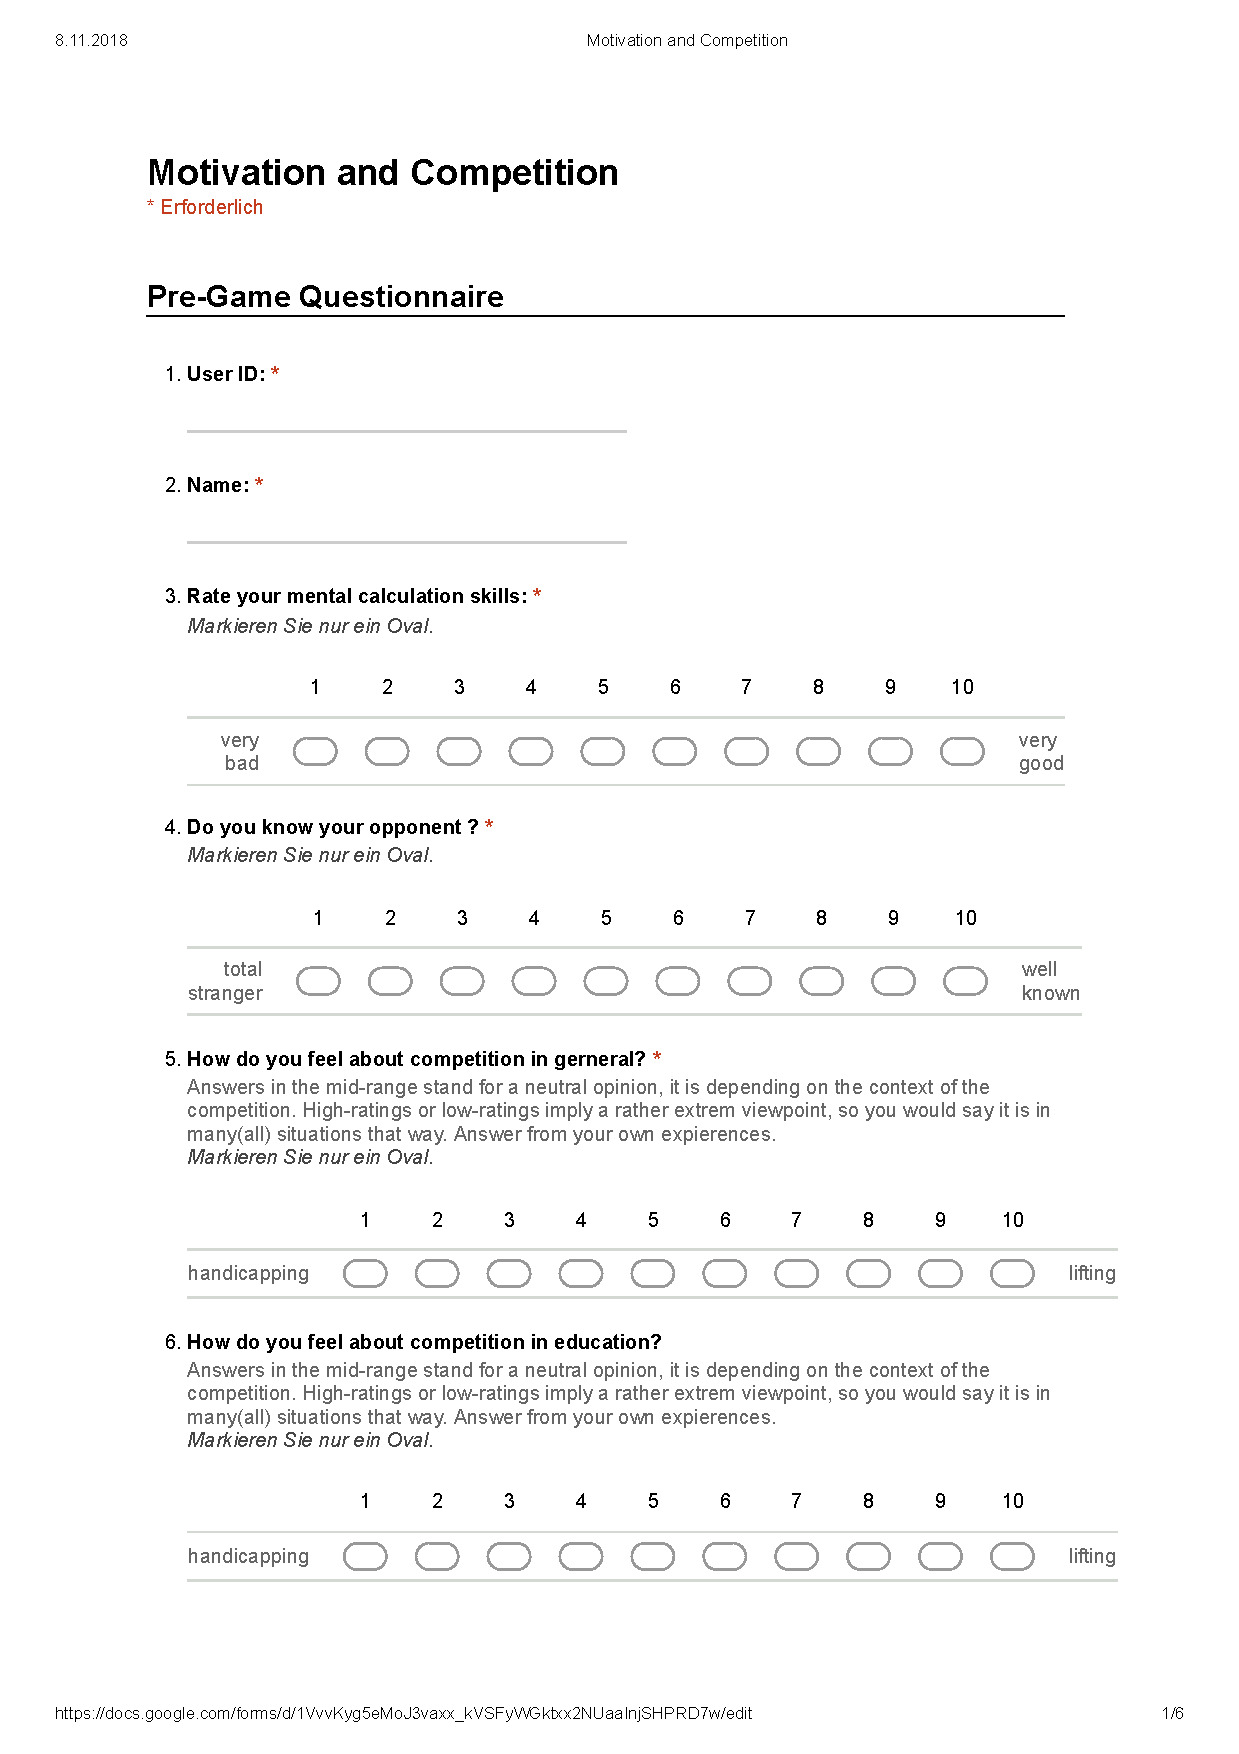
\includepdf[pages=-]{./Ressourcen/questionnaire.pdf}
\bibliography{Bibliographie}
\listoffigures

\end{document}
